% Cole Nielsen niels538@umn.edu
% EE 2002 Spring 2015
% Formal Lab Report 1

%----------------------------------------------------------------------------------------
%	PACKAGES AND DOCUMENT CONFIGURATIONS
%----------------------------------------------------------------------------------------

\documentclass[12pt]{article}

\usepackage{circuitikz}
\usepackage{graphicx}
\usepackage{subcaption}
\usepackage[top=1in, bottom= 1in, left=1in, right= 1in]{geometry}
\setlength\parindent{0pt}
\usepackage{fancyhdr}
\pagestyle{fancy}
\usepackage{textcomp}
\usepackage{tikz}
\usepackage{siunitx}
\usepackage{placeins}
\usepackage{titlesec}
\usepackage{cancel} 

%----------------------------------------------------------------------------------------
%	DOCUMENT INFORMATION
%----------------------------------------------------------------------------------------

\title{Experiment N\textsuperscript{\underline{o}} 1:   \\ Frequency Response \\and Filters\\ \vspace{0.3 in} EE 3101}

\author{Cole \textsc{Nielsen}} 
\date{Fall 2015}

\newcommand{\mymeter}[2]{   	% #1 = name , #2 = rotation angle
 \begin{scope}[transform shape,rotate=#2]
   \draw[thick] (#1)node(){$\mathbf V$} circle (11pt);
   \draw[rotate=45,-latex] (#1)  +(-17pt,0) --+(17pt,0);
 \end{scope}
}

\begin{document}
\maketitle 

\begin{center}
 \begin{tabular}{l r}
   Dates Performed: & Sept. 16 \& 23, 2015 \\ 
   Instructor: & Kyle Fox \\ 
\end{tabular}
\end{center}
\pagebreak
%----------------------------------------------------------------------------------------
%	Abstract
%----------------------------------------------------------------------------------------
\begin{abstract}
\noindent The frequency response and filter behavior of several resistor, capacitor and inductor containing circuits was tested in this lab experiment. The tendency of resistor and capacitor (RC) circuits to form low pass and high pass filters was observed. The tendency of resistor, capacitor and inductor (RLC) containing circuits to have a resonant frequency  dependent on L and C (and R if the damping is large enough) was also observed. Near the resonance frequency the RLC circuits were seen to filter input signals by either blocking a band (band reject filter) or by passing a band (band pass filter). Another observation made was a band pass filter with a low Q value can be used to produce to low pass filter with superior characteristics than a RC filter, including faster roll of and a sharper corner at the frequency cutoff. The low pass RLC circuit was even found to behave as an integrator for input signals. All circuits tested were found to confirm circuit theory, as the theoretical calculations performed matched the experimental results given some uncertainty in the results and experimental methods.
\end{abstract}
\hrulefill
%----------------------------------------------------------------------------------------
%	Introduction
%----------------------------------------------------------------------------------------
\section{Introduction}
%
In the study and application of Electrical Engineering, frequency response and filter behavior of resistor, capacitor and inductor containing circuits is of great interest. Frequency response refers to the output behavior of a system or circuit to different input frequencies. In electronics, the signal gain and phase shift of a signal due to its frequency are typically of most interest. The frequency response of these parameters are typically exhibited using what is called a Bode Plot. A Bode plot is a graph which the output parameter (e.g. phase or gain) is plotted against the input frequency of the system on a logarithmic scale. The Bode plot allows for several things, one important one being the response of filters typically graph out as linear, and another is that the response can be analyzed over large frequency ranges more effectively. \\\par

Frequency response analysis of circuits is often of most interest in the design of filters. Filters are circuits that "filter", or in other words block and pass certain ranges of input frequencies. A common topology for passive filter design makes use of a voltage divider comprised of resistors, capacitors and inductors. In short, this type of filter can be generalized by the following circuit, where $Z_1$ and $Z_2$ are some complex impedance formed by RLC components (the following will be a walk through of solving for frequency response of these types of circuits):

\begin{figure}
\begin{center}
 \begin{circuitikz}[american voltages]

   \draw
   (0,3) to[european resistor, l_=$Z_1$, o-] (3,3)
   (3,3) to[european resistor, l_=$Z_2$ ] (3,0)
         to[short, -o] (0,0)
   (3,3) to[short, -o] (4,3)      
   (3,0) to[short, -o] (4,0)
   (0,0) to[open, v^>=$v_{in}$] (0,3)
   (4,0) to[open, v_>=$v_{out}$] (4,3);
 \end{circuitikz}
 \caption[Circuit Caption]{Voltage Divider Filter}
 \end{center}
\end{figure}
\FloatBarrier
It is well known that the output voltage of such a voltage divider is as follows:
\begin{equation}
	v_{out} = v_{in} \frac{Z_2}{Z_1 + Z_2}
\end{equation}
It is helpful to think of this circuit in terms of a transfer function $H$, such that $v_{in} = H v_{out}$, which rearranges to $H = \frac{v_{out}}{v_{in}}$. Applying this to the voltage divider, it can be seen that its transfer function is as follows:
\begin{equation}
	H = \frac{Z_2}{Z_1 + Z_2}
\end{equation}
Now, consider if either $Z_1$ or $Z_2$ is complex, that is containing some inductive or capacitive component. This can complicate solving for the transfer function, so a way to simplify this is by analyzing the circuit in the Laplace domain. The impedance of resistors, capacitors and inductors in the s-domain is given as follows:
\begin{equation}
Z_R = R \hspace{24pt} Z_C = \frac{1}{sC} \hspace{24pt} Z_L = sL
\end{equation}
Solving the voltage divider transfer function with these as the impedances results in a new transfer function  in the s-domain $H(s)$. The frequency response can be directly solved from this function by plugging in $j\omega$ (the s-domain is in terms of complex frequency). The phase response can be calculated simply as the angle of the phasor formed by the real and complex parts of $H(j\omega)$. More significant in filter analysis is the gain response, which is found by taking the magnitude of $H(j\omega)$:
\begin{equation}
|H(\omega)| =\sqrt{H(j \omega) \ast H(-j \omega)}
\end{equation}
Solving for this gives a function for frequency response, which can be plotted as a Bode plot by using logarithmic scales. By trying different combinations of R and C components, it will be observed that high pass and low pass filters will be formed, where the gain will either decrease with frequency or increase with it. RLC combinations will result in band pass or band reject filters, where input frequencies will either be passed or rejected near a resonance frequency determined by the L and C values, and will be seen in the transfer function as a spike or dip at some frequency.

Understanding this, it is easy to understand the value importance of frequency response and filters in electronics, particularly in areas of telecommunication, audio, and signal processing. Filters enable the modern world of wireless communications by allowing devices such as cell phones to filter out specific frequency bands, allowing for the frequency spectrum to be shared by all. Filters even allow for audio signals to be broken down into their components, such as bass, so that it can be played through a subwoofer, or to adjust different frequency contents of the sound to be more pleasing.

Following those motivations for understanding circuit frequency response and filters, this experiment will be focused on analyzing the behavior of R, L and C filter circuits in order to gain a practical understanding of them and their application. This will be done by theoretically designing filters, constructing the circuits, testing them and validating the theory and observing any shortfalls. First, low pass and high pass filters will be considered, followed by band pass and band reject filters.
\FloatBarrier
%----------------------------------------------------------------------------------------
%	Experiment
%----------------------------------------------------------------------------------------

\section{Experiment}
\subsection*{Part 1- RC Low Pass Filter}
The RC low-pass filter below in \textit{Figure 2} was considered in this part. The objective was to design and construct the low pass filter with a corner frequency of 2 kHz, and a impedance of 10k$\Omega$ at a high frequency. From there the magnitude (gain) and phase response of the circuit was measured from 200 Hz to 20 kHz, and the experimental cut-off frequency and 45\textdegree\space phase shift frequency were determined.
\begin{figure}[h!]
\begin{center}
 \begin{circuitikz}[american voltages]
   \draw
   (0,3) to[resistor, l_=$R$, o-] (3,3)
   (3,3) to[capacitor, l_=$C$ ] (3,0)
         to[short, -o] (0,0)
   (3,3) to[short, -o] (4,3)      
   (3,0) to[short, -o] (4,0)
   (0,0) to[open, v^>=$v_{in}$] (0,3)
   (4,0) to[open, v_>=$v_{out}$] (4,3);
 \end{circuitikz}
\end{center}
\caption{RC Low Pass Filter}
\end{figure}
\FloatBarrier
\textbf{Prediction/Calculations:}
The transfer function $H(s)$ for this circuit is:
\begin{equation}
	H(s) = \frac{\frac{1}{sC}}{\frac{1}{sC} + R}
\end{equation}
Solving for $|H(j\omega)|$ 	gives
\begin{equation}
|H(j\omega)| = \frac{\frac{1}{RC}}{\sqrt{\omega^2 + \frac{1}{R^2C^2}}}
\end{equation}
The cutoff frequency $\omega_c$ occurs when the output power is halved (assuming resistive load), so $|H(j\omega_c)|$ = $\frac{\sqrt{2}}{2}|H|_{max}$, again solving this out $\omega_c$ is found to be:
\begin{equation}
\omega_c = \frac{1}{RC}
\end{equation}
The value for R is known, as the impedance of the circuit is 10k$\Omega$ at a high frequency, i.e. $Z_C$ is zero and R is equal to 10k$\Omega$. Now C can be found:
\begin{equation}
C = \frac{1}{2\pi f R} = \frac{1}{2\pi\times 2000 \times 10^4} = 7.96 nF
\end{equation}
7.96 nF is not a standard value, so two 10nF capacitors are put in series to get 5nF, and then three 1nF capacitors are added in parallel to net 8nF $\approx$ 7.96nF.\\\par

\textbf{Experiment-} The circuit was constructed on a bread board and the function generator with 2 volt peak-peak amplitude was hooked up across the $v_{in}$ terminals. The oscilloscope was connected to the circuit input on channel one and the output on channel two using grabber terminated BNC cables. The data for magnitude and phase  was measured at 15 frequencies, separated to give a relatively even spread on a log scale on the frequency range measured. The function generator amplitude was adjusted between every measurement to ensure 2 volt p-p input amplitude.\\\par

\textbf{Data-} The results for magnitude were normalized to 1, and then converted to decibels. The phase and magnitude data was then plotted as Bode Plots.
\FloatBarrier
\begin{figure}[h!]
\begin{center}
    	\resizebox{0.6\textwidth}{!}{% GNUPLOT: LaTeX picture
\setlength{\unitlength}{0.240900pt}
\ifx\plotpoint\undefined\newsavebox{\plotpoint}\fi
\begin{picture}(1500,900)(0,0)
\sbox{\plotpoint}{\rule[-0.200pt]{0.400pt}{0.400pt}}%
\put(151.0,131.0){\rule[-0.200pt]{4.818pt}{0.400pt}}
\put(131,131){\makebox(0,0)[r]{-20}}
\put(1419.0,131.0){\rule[-0.200pt]{4.818pt}{0.400pt}}
\put(151.0,196.0){\rule[-0.200pt]{4.818pt}{0.400pt}}
\put(131,196){\makebox(0,0)[r]{-18}}
\put(1419.0,196.0){\rule[-0.200pt]{4.818pt}{0.400pt}}
\put(151.0,260.0){\rule[-0.200pt]{4.818pt}{0.400pt}}
\put(131,260){\makebox(0,0)[r]{-16}}
\put(1419.0,260.0){\rule[-0.200pt]{4.818pt}{0.400pt}}
\put(151.0,325.0){\rule[-0.200pt]{4.818pt}{0.400pt}}
\put(131,325){\makebox(0,0)[r]{-14}}
\put(1419.0,325.0){\rule[-0.200pt]{4.818pt}{0.400pt}}
\put(151.0,389.0){\rule[-0.200pt]{4.818pt}{0.400pt}}
\put(131,389){\makebox(0,0)[r]{-12}}
\put(1419.0,389.0){\rule[-0.200pt]{4.818pt}{0.400pt}}
\put(151.0,454.0){\rule[-0.200pt]{4.818pt}{0.400pt}}
\put(131,454){\makebox(0,0)[r]{-10}}
\put(1419.0,454.0){\rule[-0.200pt]{4.818pt}{0.400pt}}
\put(151.0,518.0){\rule[-0.200pt]{4.818pt}{0.400pt}}
\put(131,518){\makebox(0,0)[r]{-8}}
\put(1419.0,518.0){\rule[-0.200pt]{4.818pt}{0.400pt}}
\put(151.0,583.0){\rule[-0.200pt]{4.818pt}{0.400pt}}
\put(131,583){\makebox(0,0)[r]{-6}}
\put(1419.0,583.0){\rule[-0.200pt]{4.818pt}{0.400pt}}
\put(151.0,647.0){\rule[-0.200pt]{4.818pt}{0.400pt}}
\put(131,647){\makebox(0,0)[r]{-4}}
\put(1419.0,647.0){\rule[-0.200pt]{4.818pt}{0.400pt}}
\put(151.0,712.0){\rule[-0.200pt]{4.818pt}{0.400pt}}
\put(131,712){\makebox(0,0)[r]{-2}}
\put(1419.0,712.0){\rule[-0.200pt]{4.818pt}{0.400pt}}
\put(151.0,776.0){\rule[-0.200pt]{4.818pt}{0.400pt}}
\put(131,776){\makebox(0,0)[r]{ 0}}
\put(1419.0,776.0){\rule[-0.200pt]{4.818pt}{0.400pt}}
\put(151.0,131.0){\rule[-0.200pt]{0.400pt}{4.818pt}}
\put(151,90){\makebox(0,0){ 200}}
\put(151.0,756.0){\rule[-0.200pt]{0.400pt}{4.818pt}}
\put(345.0,131.0){\rule[-0.200pt]{0.400pt}{4.818pt}}
\put(345.0,756.0){\rule[-0.200pt]{0.400pt}{4.818pt}}
\put(458.0,131.0){\rule[-0.200pt]{0.400pt}{4.818pt}}
\put(458.0,756.0){\rule[-0.200pt]{0.400pt}{4.818pt}}
\put(539.0,131.0){\rule[-0.200pt]{0.400pt}{4.818pt}}
\put(539.0,756.0){\rule[-0.200pt]{0.400pt}{4.818pt}}
\put(601.0,131.0){\rule[-0.200pt]{0.400pt}{4.818pt}}
\put(601.0,756.0){\rule[-0.200pt]{0.400pt}{4.818pt}}
\put(652.0,131.0){\rule[-0.200pt]{0.400pt}{4.818pt}}
\put(652.0,756.0){\rule[-0.200pt]{0.400pt}{4.818pt}}
\put(695.0,131.0){\rule[-0.200pt]{0.400pt}{4.818pt}}
\put(695.0,756.0){\rule[-0.200pt]{0.400pt}{4.818pt}}
\put(733.0,131.0){\rule[-0.200pt]{0.400pt}{4.818pt}}
\put(733.0,756.0){\rule[-0.200pt]{0.400pt}{4.818pt}}
\put(766.0,131.0){\rule[-0.200pt]{0.400pt}{4.818pt}}
\put(766.0,756.0){\rule[-0.200pt]{0.400pt}{4.818pt}}
\put(795.0,131.0){\rule[-0.200pt]{0.400pt}{4.818pt}}
\put(795,90){\makebox(0,0){ 2000}}
\put(795.0,756.0){\rule[-0.200pt]{0.400pt}{4.818pt}}
\put(989.0,131.0){\rule[-0.200pt]{0.400pt}{4.818pt}}
\put(989.0,756.0){\rule[-0.200pt]{0.400pt}{4.818pt}}
\put(1102.0,131.0){\rule[-0.200pt]{0.400pt}{4.818pt}}
\put(1102.0,756.0){\rule[-0.200pt]{0.400pt}{4.818pt}}
\put(1183.0,131.0){\rule[-0.200pt]{0.400pt}{4.818pt}}
\put(1183.0,756.0){\rule[-0.200pt]{0.400pt}{4.818pt}}
\put(1245.0,131.0){\rule[-0.200pt]{0.400pt}{4.818pt}}
\put(1245.0,756.0){\rule[-0.200pt]{0.400pt}{4.818pt}}
\put(1296.0,131.0){\rule[-0.200pt]{0.400pt}{4.818pt}}
\put(1296.0,756.0){\rule[-0.200pt]{0.400pt}{4.818pt}}
\put(1339.0,131.0){\rule[-0.200pt]{0.400pt}{4.818pt}}
\put(1339.0,756.0){\rule[-0.200pt]{0.400pt}{4.818pt}}
\put(1377.0,131.0){\rule[-0.200pt]{0.400pt}{4.818pt}}
\put(1377.0,756.0){\rule[-0.200pt]{0.400pt}{4.818pt}}
\put(1410.0,131.0){\rule[-0.200pt]{0.400pt}{4.818pt}}
\put(1410.0,756.0){\rule[-0.200pt]{0.400pt}{4.818pt}}
\put(1439.0,131.0){\rule[-0.200pt]{0.400pt}{4.818pt}}
\put(1439,90){\makebox(0,0){ 20000}}
\put(1439.0,756.0){\rule[-0.200pt]{0.400pt}{4.818pt}}
\put(151.0,131.0){\rule[-0.200pt]{0.400pt}{155.380pt}}
\put(151.0,131.0){\rule[-0.200pt]{310.279pt}{0.400pt}}
\put(1439.0,131.0){\rule[-0.200pt]{0.400pt}{155.380pt}}
\put(151.0,776.0){\rule[-0.200pt]{310.279pt}{0.400pt}}
\put(30,453){\makebox(0,0){\hspace{-48pt}Gain (dB)}}
\put(795,29){\makebox(0,0){Frequency (Hz)}}
\put(795,838){\makebox(0,0){RC Low Pass Filter Gain vs. Frequency}}
\put(151,776){\makebox(0,0){$+$}}
\put(458,764){\makebox(0,0){$+$}}
\put(601,746){\makebox(0,0){$+$}}
\put(695,726){\makebox(0,0){$+$}}
\put(733,712){\makebox(0,0){$+$}}
\put(766,705){\makebox(0,0){$+$}}
\put(795,690){\makebox(0,0){$+$}}
\put(822,674){\makebox(0,0){$+$}}
\put(846,665){\makebox(0,0){$+$}}
\put(889,639){\makebox(0,0){$+$}}
\put(989,564){\makebox(0,0){$+$}}
\put(1102,479){\makebox(0,0){$+$}}
\put(1183,404){\makebox(0,0){$+$}}
\put(1296,331){\makebox(0,0){$+$}}
\put(1377,231){\makebox(0,0){$+$}}
\put(1439,158){\makebox(0,0){$+$}}
\put(812,680){\makebox(0,0){$\bullet$}}
\put(1000,720){\makebox(0,0){(2.11 kHz, -3dB)}}
\put(151,776){\usebox{\plotpoint}}
\multiput(151.00,774.92)(13.205,-0.492){21}{\rule{10.333pt}{0.119pt}}
\multiput(151.00,775.17)(285.553,-12.000){2}{\rule{5.167pt}{0.400pt}}
\multiput(458.00,762.92)(4.044,-0.495){33}{\rule{3.278pt}{0.119pt}}
\multiput(458.00,763.17)(136.197,-18.000){2}{\rule{1.639pt}{0.400pt}}
\multiput(601.00,744.92)(2.383,-0.496){37}{\rule{1.980pt}{0.119pt}}
\multiput(601.00,745.17)(89.890,-20.000){2}{\rule{0.990pt}{0.400pt}}
\multiput(695.00,724.92)(1.378,-0.494){25}{\rule{1.186pt}{0.119pt}}
\multiput(695.00,725.17)(35.539,-14.000){2}{\rule{0.593pt}{0.400pt}}
\multiput(733.00,710.93)(2.476,-0.485){11}{\rule{1.986pt}{0.117pt}}
\multiput(733.00,711.17)(28.879,-7.000){2}{\rule{0.993pt}{0.400pt}}
\multiput(766.00,703.92)(0.976,-0.494){27}{\rule{0.873pt}{0.119pt}}
\multiput(766.00,704.17)(27.187,-15.000){2}{\rule{0.437pt}{0.400pt}}
\multiput(795.00,688.92)(0.849,-0.494){29}{\rule{0.775pt}{0.119pt}}
\multiput(795.00,689.17)(25.391,-16.000){2}{\rule{0.388pt}{0.400pt}}
\multiput(822.00,672.93)(1.368,-0.489){15}{\rule{1.167pt}{0.118pt}}
\multiput(822.00,673.17)(21.579,-9.000){2}{\rule{0.583pt}{0.400pt}}
\multiput(846.00,663.92)(0.830,-0.497){49}{\rule{0.762pt}{0.120pt}}
\multiput(846.00,664.17)(41.419,-26.000){2}{\rule{0.381pt}{0.400pt}}
\multiput(889.00,637.92)(0.667,-0.499){147}{\rule{0.633pt}{0.120pt}}
\multiput(889.00,638.17)(98.685,-75.000){2}{\rule{0.317pt}{0.400pt}}
\multiput(989.00,562.92)(0.665,-0.499){167}{\rule{0.632pt}{0.120pt}}
\multiput(989.00,563.17)(111.689,-85.000){2}{\rule{0.316pt}{0.400pt}}
\multiput(1102.00,477.92)(0.540,-0.499){147}{\rule{0.532pt}{0.120pt}}
\multiput(1102.00,478.17)(79.896,-75.000){2}{\rule{0.266pt}{0.400pt}}
\multiput(1183.00,402.92)(0.775,-0.499){143}{\rule{0.719pt}{0.120pt}}
\multiput(1183.00,403.17)(111.507,-73.000){2}{\rule{0.360pt}{0.400pt}}
\multiput(1296.58,328.53)(0.499,-0.617){159}{\rule{0.120pt}{0.594pt}}
\multiput(1295.17,329.77)(81.000,-98.767){2}{\rule{0.400pt}{0.297pt}}
\multiput(1377.58,228.63)(0.499,-0.589){121}{\rule{0.120pt}{0.571pt}}
\multiput(1376.17,229.81)(62.000,-71.815){2}{\rule{0.400pt}{0.285pt}}
\sbox{\plotpoint}{\rule[-0.500pt]{1.000pt}{1.000pt}}%
\put(810,131){\usebox{\plotpoint}}
\multiput(810,131)(0.000,20.756){27}{\usebox{\plotpoint}}
\put(810,679){\usebox{\plotpoint}}
\multiput(151,679)(20.756,0.000){32}{\usebox{\plotpoint}}
\put(810,679){\usebox{\plotpoint}}
\sbox{\plotpoint}{\rule[-0.200pt]{0.400pt}{0.400pt}}%
\put(151.0,131.0){\rule[-0.200pt]{0.400pt}{155.380pt}}
\put(151.0,131.0){\rule[-0.200pt]{310.279pt}{0.400pt}}
\put(1439.0,131.0){\rule[-0.200pt]{0.400pt}{155.380pt}}
\put(151.0,776.0){\rule[-0.200pt]{310.279pt}{0.400pt}}
\end{picture}
}
\end{center}
\caption{RC Low Pass Filter Gain Bode Plot\\ Cut-off Frequency (-3dB point) : 2.11 kHz}
\end{figure}
\begin{figure}[h!]

\begin{center}
    	\resizebox{0.6\textwidth}{!}{% GNUPLOT: LaTeX picture
\setlength{\unitlength}{0.240900pt}
\ifx\plotpoint\undefined\newsavebox{\plotpoint}\fi
\sbox{\plotpoint}{\rule[-0.200pt]{0.400pt}{0.400pt}}%
\begin{picture}(1500,900)(0,0)
\sbox{\plotpoint}{\rule[-0.200pt]{0.400pt}{0.400pt}}%
\put(151.0,131.0){\rule[-0.200pt]{4.818pt}{0.400pt}}
\put(131,131){\makebox(0,0)[r]{-90}}
\put(1419.0,131.0){\rule[-0.200pt]{4.818pt}{0.400pt}}
\put(151.0,203.0){\rule[-0.200pt]{4.818pt}{0.400pt}}
\put(131,203){\makebox(0,0)[r]{-80}}
\put(1419.0,203.0){\rule[-0.200pt]{4.818pt}{0.400pt}}
\put(151.0,274.0){\rule[-0.200pt]{4.818pt}{0.400pt}}
\put(131,274){\makebox(0,0)[r]{-70}}
\put(1419.0,274.0){\rule[-0.200pt]{4.818pt}{0.400pt}}
\put(151.0,346.0){\rule[-0.200pt]{4.818pt}{0.400pt}}
\put(131,346){\makebox(0,0)[r]{-60}}
\put(1419.0,346.0){\rule[-0.200pt]{4.818pt}{0.400pt}}
\put(151.0,418.0){\rule[-0.200pt]{4.818pt}{0.400pt}}
\put(131,418){\makebox(0,0)[r]{-50}}
\put(1419.0,418.0){\rule[-0.200pt]{4.818pt}{0.400pt}}
\put(151.0,489.0){\rule[-0.200pt]{4.818pt}{0.400pt}}
\put(131,489){\makebox(0,0)[r]{-40}}
\put(1419.0,489.0){\rule[-0.200pt]{4.818pt}{0.400pt}}
\put(151.0,561.0){\rule[-0.200pt]{4.818pt}{0.400pt}}
\put(131,561){\makebox(0,0)[r]{-30}}
\put(1419.0,561.0){\rule[-0.200pt]{4.818pt}{0.400pt}}
\put(151.0,633.0){\rule[-0.200pt]{4.818pt}{0.400pt}}
\put(131,633){\makebox(0,0)[r]{-20}}
\put(1419.0,633.0){\rule[-0.200pt]{4.818pt}{0.400pt}}
\put(151.0,704.0){\rule[-0.200pt]{4.818pt}{0.400pt}}
\put(131,704){\makebox(0,0)[r]{-10}}
\put(1419.0,704.0){\rule[-0.200pt]{4.818pt}{0.400pt}}
\put(151.0,776.0){\rule[-0.200pt]{4.818pt}{0.400pt}}
\put(131,776){\makebox(0,0)[r]{ 0}}
\put(1419.0,776.0){\rule[-0.200pt]{4.818pt}{0.400pt}}
\put(151.0,131.0){\rule[-0.200pt]{0.400pt}{4.818pt}}
\put(151,90){\makebox(0,0){ 200}}
\put(151.0,756.0){\rule[-0.200pt]{0.400pt}{4.818pt}}
\put(345.0,131.0){\rule[-0.200pt]{0.400pt}{4.818pt}}
\put(345.0,756.0){\rule[-0.200pt]{0.400pt}{4.818pt}}
\put(458.0,131.0){\rule[-0.200pt]{0.400pt}{4.818pt}}
\put(458.0,756.0){\rule[-0.200pt]{0.400pt}{4.818pt}}
\put(539.0,131.0){\rule[-0.200pt]{0.400pt}{4.818pt}}
\put(539.0,756.0){\rule[-0.200pt]{0.400pt}{4.818pt}}
\put(601.0,131.0){\rule[-0.200pt]{0.400pt}{4.818pt}}
\put(601.0,756.0){\rule[-0.200pt]{0.400pt}{4.818pt}}
\put(652.0,131.0){\rule[-0.200pt]{0.400pt}{4.818pt}}
\put(652.0,756.0){\rule[-0.200pt]{0.400pt}{4.818pt}}
\put(695.0,131.0){\rule[-0.200pt]{0.400pt}{4.818pt}}
\put(695.0,756.0){\rule[-0.200pt]{0.400pt}{4.818pt}}
\put(733.0,131.0){\rule[-0.200pt]{0.400pt}{4.818pt}}
\put(733.0,756.0){\rule[-0.200pt]{0.400pt}{4.818pt}}
\put(766.0,131.0){\rule[-0.200pt]{0.400pt}{4.818pt}}
\put(766.0,756.0){\rule[-0.200pt]{0.400pt}{4.818pt}}
\put(795.0,131.0){\rule[-0.200pt]{0.400pt}{4.818pt}}
\put(795,90){\makebox(0,0){ 2000}}
\put(795.0,756.0){\rule[-0.200pt]{0.400pt}{4.818pt}}
\put(989.0,131.0){\rule[-0.200pt]{0.400pt}{4.818pt}}
\put(989.0,756.0){\rule[-0.200pt]{0.400pt}{4.818pt}}
\put(1102.0,131.0){\rule[-0.200pt]{0.400pt}{4.818pt}}
\put(1102.0,756.0){\rule[-0.200pt]{0.400pt}{4.818pt}}
\put(1183.0,131.0){\rule[-0.200pt]{0.400pt}{4.818pt}}
\put(1183.0,756.0){\rule[-0.200pt]{0.400pt}{4.818pt}}
\put(1245.0,131.0){\rule[-0.200pt]{0.400pt}{4.818pt}}
\put(1245.0,756.0){\rule[-0.200pt]{0.400pt}{4.818pt}}
\put(1296.0,131.0){\rule[-0.200pt]{0.400pt}{4.818pt}}
\put(1296.0,756.0){\rule[-0.200pt]{0.400pt}{4.818pt}}
\put(1339.0,131.0){\rule[-0.200pt]{0.400pt}{4.818pt}}
\put(1339.0,756.0){\rule[-0.200pt]{0.400pt}{4.818pt}}
\put(1377.0,131.0){\rule[-0.200pt]{0.400pt}{4.818pt}}
\put(1377.0,756.0){\rule[-0.200pt]{0.400pt}{4.818pt}}
\put(1410.0,131.0){\rule[-0.200pt]{0.400pt}{4.818pt}}
\put(1410.0,756.0){\rule[-0.200pt]{0.400pt}{4.818pt}}
\put(1439.0,131.0){\rule[-0.200pt]{0.400pt}{4.818pt}}
\put(1439,90){\makebox(0,0){ 20000}}
\put(1439.0,756.0){\rule[-0.200pt]{0.400pt}{4.818pt}}
\put(151.0,131.0){\rule[-0.200pt]{0.400pt}{155.380pt}}
\put(151.0,131.0){\rule[-0.200pt]{310.279pt}{0.400pt}}
\put(1439.0,131.0){\rule[-0.200pt]{0.400pt}{155.380pt}}
\put(151.0,776.0){\rule[-0.200pt]{310.279pt}{0.400pt}}
\put(30,453){\makebox(0,0){\hspace{-72pt}Phase (degrees)}}
\put(795,29){\makebox(0,0){Frequency (Hz)}}
\put(795,838){\makebox(0,0){RC Low Pass Filter Phase vs. Frequency}}
\put(151,741){\makebox(0,0){$+$}}
\put(458,656){\makebox(0,0){$+$}}
\put(601,593){\makebox(0,0){$+$}}
\put(695,537){\makebox(0,0){$+$}}
\put(733,516){\makebox(0,0){$+$}}
\put(766,493){\makebox(0,0){$+$}}
\put(795,471){\makebox(0,0){$+$}}
\put(810,454){\makebox(0,0){$\bullet$}}
\put(990,500){\makebox(0,0){(2.11 kHz, -45\textdegree)}}
\put(822,446){\makebox(0,0){$+$}}
\put(846,431){\makebox(0,0){$+$}}
\put(889,400){\makebox(0,0){$+$}}
\put(989,355){\makebox(0,0){$+$}}
\put(1102,282){\makebox(0,0){$+$}}
\put(1183,250){\makebox(0,0){$+$}}
\put(1296,210){\makebox(0,0){$+$}}
\put(1377,188){\makebox(0,0){$+$}}
\put(1439,167){\makebox(0,0){$+$}}
\put(151,741){\usebox{\plotpoint}}
\multiput(151.00,739.92)(1.811,-0.499){167}{\rule{1.545pt}{0.120pt}}
\multiput(151.00,740.17)(303.794,-85.000){2}{\rule{0.772pt}{0.400pt}}
\multiput(458.00,654.92)(1.138,-0.499){123}{\rule{1.008pt}{0.120pt}}
\multiput(458.00,655.17)(140.908,-63.000){2}{\rule{0.504pt}{0.400pt}}
\multiput(601.00,591.92)(0.841,-0.499){109}{\rule{0.771pt}{0.120pt}}
\multiput(601.00,592.17)(92.399,-56.000){2}{\rule{0.386pt}{0.400pt}}
\multiput(695.00,535.92)(0.910,-0.496){39}{\rule{0.824pt}{0.119pt}}
\multiput(695.00,536.17)(36.290,-21.000){2}{\rule{0.412pt}{0.400pt}}
\multiput(733.00,514.92)(0.719,-0.496){43}{\rule{0.674pt}{0.120pt}}
\multiput(733.00,515.17)(31.601,-23.000){2}{\rule{0.337pt}{0.400pt}}
\multiput(766.00,491.92)(0.660,-0.496){41}{\rule{0.627pt}{0.120pt}}
\multiput(766.00,492.17)(27.698,-22.000){2}{\rule{0.314pt}{0.400pt}}
\multiput(795.58,468.70)(0.494,-0.566){27}{\rule{0.119pt}{0.553pt}}
\multiput(794.17,469.85)(15.000,-15.852){2}{\rule{0.400pt}{0.277pt}}
\multiput(810.00,452.93)(0.758,-0.488){13}{\rule{0.700pt}{0.117pt}}
\multiput(810.00,453.17)(10.547,-8.000){2}{\rule{0.350pt}{0.400pt}}
\multiput(822.00,444.92)(0.805,-0.494){27}{\rule{0.740pt}{0.119pt}}
\multiput(822.00,445.17)(22.464,-15.000){2}{\rule{0.370pt}{0.400pt}}
\multiput(846.00,429.92)(0.695,-0.497){59}{\rule{0.655pt}{0.120pt}}
\multiput(846.00,430.17)(41.641,-31.000){2}{\rule{0.327pt}{0.400pt}}
\multiput(889.00,398.92)(1.115,-0.498){87}{\rule{0.989pt}{0.120pt}}
\multiput(889.00,399.17)(97.948,-45.000){2}{\rule{0.494pt}{0.400pt}}
\multiput(989.00,353.92)(0.775,-0.499){143}{\rule{0.719pt}{0.120pt}}
\multiput(989.00,354.17)(111.507,-73.000){2}{\rule{0.360pt}{0.400pt}}
\multiput(1102.00,280.92)(1.273,-0.497){61}{\rule{1.112pt}{0.120pt}}
\multiput(1102.00,281.17)(78.691,-32.000){2}{\rule{0.556pt}{0.400pt}}
\multiput(1183.00,248.92)(1.420,-0.498){77}{\rule{1.230pt}{0.120pt}}
\multiput(1183.00,249.17)(110.447,-40.000){2}{\rule{0.615pt}{0.400pt}}
\multiput(1296.00,208.92)(1.862,-0.496){41}{\rule{1.573pt}{0.120pt}}
\multiput(1296.00,209.17)(77.736,-22.000){2}{\rule{0.786pt}{0.400pt}}
\multiput(1377.00,186.92)(1.492,-0.496){39}{\rule{1.281pt}{0.119pt}}
\multiput(1377.00,187.17)(59.341,-21.000){2}{\rule{0.640pt}{0.400pt}}
\sbox{\plotpoint}{\rule[-0.500pt]{1.000pt}{1.000pt}}%
\put(151,454){\usebox{\plotpoint}}
\multiput(151,454)(20.756,0.000){32}{\usebox{\plotpoint}}
\put(810,454){\usebox{\plotpoint}}
\put(810,131){\usebox{\plotpoint}}
\multiput(810,131)(0.000,20.756){16}{\usebox{\plotpoint}}
\put(810,454){\usebox{\plotpoint}}
\sbox{\plotpoint}{\rule[-0.200pt]{0.400pt}{0.400pt}}%
\put(151.0,131.0){\rule[-0.200pt]{0.400pt}{155.380pt}}
\put(151.0,131.0){\rule[-0.200pt]{310.279pt}{0.400pt}}
\put(1439.0,131.0){\rule[-0.200pt]{0.400pt}{155.380pt}}
\put(151.0,776.0){\rule[-0.200pt]{310.279pt}{0.400pt}}
\end{picture}
}
\end{center}
\caption{RC Low Pass Filter Phase Bode Plot \\ 45\textdegree\space Phase Shift Frequency: 2.11 kHz}
\end{figure}
\FloatBarrier
\textbf{Conclusion-} The filter behaved as expected as a low pass filter, having its cut-off point at 2.11 kHz, which is 5.5\% away from the theoretical 2 kHz. Given the resistor tolerance of 5\%, and the capacitor's 10\%, this error is understandable and likely attributable to the tolerances as it is less than the greatest tolerance. The frequency at which a phase shift of 45\textdegree\space occured at was also 2.11 kHz. The reason for this is logical if one looks at the phasor for the system, shown below, at the cut-off frequency. The cut-off point corresponds to half power (into a real load), which is equal to $\frac{\sqrt{2}}{2}V_{in}$. Using that relationship and simple geometry, one can calculate that the angle, or phase, between the input and output (real portion of the signal) is -45 \textdegree. Intuitively this circuit acts as a low pass filter because a capacitor conducts  more at greater frequencies, so when this circuit is thought of as a voltage divider, it makes sense that the output voltage will drop with frequency across the capacitor.
\begin{figure}[h!]
\begin{center}
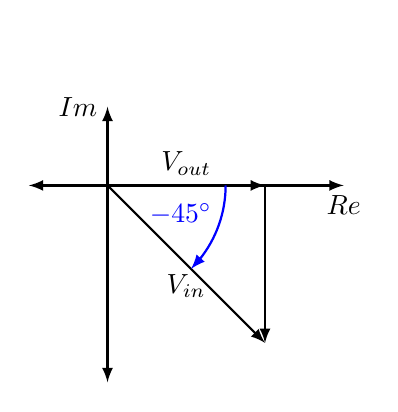
\begin{tikzpicture}[>=latex]
\draw[style=help lines] (0,0) (3,2);

\coordinate (vec1) at (315:2.828); 
\coordinate (vec2) at (30:3);
\coordinate (vec3) at (0:3);
\coordinate (vec4) at (90:1);
\coordinate (vec5) at (270:2.5);
\coordinate (vec6) at (180:1);

\draw[->,thick,black] (0,0) -- (vec1) node[midway, below] {$V_{in}$};
\draw[->,thick,black] (0,0) -- (vec3) node [below] {$Re$};
\draw[->,thick,black] (0,0) -- (vec4) node [left] {$Im$};
\draw[->,thick,black] (0,0) -- (vec5);
\draw[->,thick,black] (0,0) -- (vec6);
\draw[->,thick,black] (2,0) -- (2,-2);
\draw[->,thick,black] (0,0) -- (2,0) node [midway, above] {$V_{out}$};

\draw [->, blue, thick] (1.5,0) arc [start angle=0, end angle=-45, radius=1.5cm]
    node [right, near start] {}; 
\node [blue, thick] at (.93,-0.37) {$\ang{-45}$};   
\end{tikzpicture}
\end{center}
\caption{Circuit's Phasor Diagram at Cut-off Frequency}
\end{figure}

\subsection*{Part 2- RC High Pass Filter}
The RC high pass filter of \textit{Figure 6}, being an interchanged version of the previous circuit was considered. The same values were used for all components, and the same measurements were performed.
\begin{figure}[h!]
\begin{center}
 \begin{circuitikz}[american voltages]
   \draw
   (0,3) to[capacitor, l_=8nF, o-] (3,3)
   (3,3) to[resistor, l_=10k$\Omega$ ] (3,0)
         to[short, -o] (0,0)
   (3,3) to[short, -o] (4,3)      
   (3,0) to[short, -o] (4,0)
   (0,0) to[open, v^>=$v_{in}$] (0,3)
   (4,0) to[open, v_>=$v_{out}$] (4,3);
 \end{circuitikz}
\end{center}
\caption{RC High Pass Filter}
\end{figure}
\FloatBarrier
\textbf{Prediction/Calculations-} Similar to part 1, the transfer function $H(s)$ can be found, and then $|H(j\omega)|$ following:
\begin{equation}
H(s) = \frac{R}{\frac{1}{sC} + R} \hspace{24pt} \rightarrow \hspace{24pt} |H(j\omega)| = \frac{\omega}{\sqrt{\omega^2 +\frac{1}{R^2C^2}}}
\end{equation}
The cut-off can then be found using the same methods as before, yielding:
\begin{equation}
\omega_c = \frac{1}{RC}
\end{equation} 
Since this equation is the same at part 1, we expect the same 2 kHz cutoff.\\\par 
\textbf{Experiment-} The same procedure was performed as part 1.\\\par 
\pagebreak
\textbf{Data-}

\begin{figure}[h!]
\begin{center}
    	\resizebox{0.6\textwidth}{!}{% GNUPLOT: LaTeX picture
\setlength{\unitlength}{0.240900pt}
\ifx\plotpoint\undefined\newsavebox{\plotpoint}\fi
\sbox{\plotpoint}{\rule[-0.200pt]{0.400pt}{0.400pt}}%
\begin{picture}(1500,900)(0,0)
\sbox{\plotpoint}{\rule[-0.200pt]{0.400pt}{0.400pt}}%
\put(151.0,131.0){\rule[-0.200pt]{4.818pt}{0.400pt}}
\put(131,131){\makebox(0,0)[r]{-20}}
\put(1419.0,131.0){\rule[-0.200pt]{4.818pt}{0.400pt}}
\put(151.0,196.0){\rule[-0.200pt]{4.818pt}{0.400pt}}
\put(131,196){\makebox(0,0)[r]{-18}}
\put(1419.0,196.0){\rule[-0.200pt]{4.818pt}{0.400pt}}
\put(151.0,260.0){\rule[-0.200pt]{4.818pt}{0.400pt}}
\put(131,260){\makebox(0,0)[r]{-16}}
\put(1419.0,260.0){\rule[-0.200pt]{4.818pt}{0.400pt}}
\put(151.0,325.0){\rule[-0.200pt]{4.818pt}{0.400pt}}
\put(131,325){\makebox(0,0)[r]{-14}}
\put(1419.0,325.0){\rule[-0.200pt]{4.818pt}{0.400pt}}
\put(151.0,389.0){\rule[-0.200pt]{4.818pt}{0.400pt}}
\put(131,389){\makebox(0,0)[r]{-12}}
\put(1419.0,389.0){\rule[-0.200pt]{4.818pt}{0.400pt}}
\put(151.0,454.0){\rule[-0.200pt]{4.818pt}{0.400pt}}
\put(131,454){\makebox(0,0)[r]{-10}}
\put(1419.0,454.0){\rule[-0.200pt]{4.818pt}{0.400pt}}
\put(151.0,518.0){\rule[-0.200pt]{4.818pt}{0.400pt}}
\put(131,518){\makebox(0,0)[r]{-8}}
\put(1419.0,518.0){\rule[-0.200pt]{4.818pt}{0.400pt}}
\put(151.0,583.0){\rule[-0.200pt]{4.818pt}{0.400pt}}
\put(131,583){\makebox(0,0)[r]{-6}}
\put(1419.0,583.0){\rule[-0.200pt]{4.818pt}{0.400pt}}
\put(151.0,647.0){\rule[-0.200pt]{4.818pt}{0.400pt}}
\put(131,647){\makebox(0,0)[r]{-4}}
\put(1419.0,647.0){\rule[-0.200pt]{4.818pt}{0.400pt}}
\put(151.0,712.0){\rule[-0.200pt]{4.818pt}{0.400pt}}
\put(131,712){\makebox(0,0)[r]{-2}}
\put(1419.0,712.0){\rule[-0.200pt]{4.818pt}{0.400pt}}
\put(151.0,776.0){\rule[-0.200pt]{4.818pt}{0.400pt}}
\put(131,776){\makebox(0,0)[r]{ 0}}
\put(1419.0,776.0){\rule[-0.200pt]{4.818pt}{0.400pt}}
\put(151.0,131.0){\rule[-0.200pt]{0.400pt}{4.818pt}}
\put(151,90){\makebox(0,0){ 200}}
\put(151.0,756.0){\rule[-0.200pt]{0.400pt}{4.818pt}}
\put(345.0,131.0){\rule[-0.200pt]{0.400pt}{4.818pt}}
\put(345.0,756.0){\rule[-0.200pt]{0.400pt}{4.818pt}}
\put(458.0,131.0){\rule[-0.200pt]{0.400pt}{4.818pt}}
\put(458.0,756.0){\rule[-0.200pt]{0.400pt}{4.818pt}}
\put(539.0,131.0){\rule[-0.200pt]{0.400pt}{4.818pt}}
\put(539.0,756.0){\rule[-0.200pt]{0.400pt}{4.818pt}}
\put(601.0,131.0){\rule[-0.200pt]{0.400pt}{4.818pt}}
\put(601.0,756.0){\rule[-0.200pt]{0.400pt}{4.818pt}}
\put(652.0,131.0){\rule[-0.200pt]{0.400pt}{4.818pt}}
\put(652.0,756.0){\rule[-0.200pt]{0.400pt}{4.818pt}}
\put(695.0,131.0){\rule[-0.200pt]{0.400pt}{4.818pt}}
\put(695.0,756.0){\rule[-0.200pt]{0.400pt}{4.818pt}}
\put(733.0,131.0){\rule[-0.200pt]{0.400pt}{4.818pt}}
\put(733.0,756.0){\rule[-0.200pt]{0.400pt}{4.818pt}}
\put(766.0,131.0){\rule[-0.200pt]{0.400pt}{4.818pt}}
\put(766.0,756.0){\rule[-0.200pt]{0.400pt}{4.818pt}}
\put(795.0,131.0){\rule[-0.200pt]{0.400pt}{4.818pt}}
\put(795,90){\makebox(0,0){ 2000}}
\put(795.0,756.0){\rule[-0.200pt]{0.400pt}{4.818pt}}
\put(989.0,131.0){\rule[-0.200pt]{0.400pt}{4.818pt}}
\put(989.0,756.0){\rule[-0.200pt]{0.400pt}{4.818pt}}
\put(1102.0,131.0){\rule[-0.200pt]{0.400pt}{4.818pt}}
\put(1102.0,756.0){\rule[-0.200pt]{0.400pt}{4.818pt}}
\put(1183.0,131.0){\rule[-0.200pt]{0.400pt}{4.818pt}}
\put(1183.0,756.0){\rule[-0.200pt]{0.400pt}{4.818pt}}
\put(1245.0,131.0){\rule[-0.200pt]{0.400pt}{4.818pt}}
\put(1245.0,756.0){\rule[-0.200pt]{0.400pt}{4.818pt}}
\put(1296.0,131.0){\rule[-0.200pt]{0.400pt}{4.818pt}}
\put(1296.0,756.0){\rule[-0.200pt]{0.400pt}{4.818pt}}
\put(1339.0,131.0){\rule[-0.200pt]{0.400pt}{4.818pt}}
\put(1339.0,756.0){\rule[-0.200pt]{0.400pt}{4.818pt}}
\put(1377.0,131.0){\rule[-0.200pt]{0.400pt}{4.818pt}}
\put(1377.0,756.0){\rule[-0.200pt]{0.400pt}{4.818pt}}
\put(1410.0,131.0){\rule[-0.200pt]{0.400pt}{4.818pt}}
\put(1410.0,756.0){\rule[-0.200pt]{0.400pt}{4.818pt}}
\put(1439.0,131.0){\rule[-0.200pt]{0.400pt}{4.818pt}}
\put(1439,90){\makebox(0,0){ 20000}}
\put(1439.0,756.0){\rule[-0.200pt]{0.400pt}{4.818pt}}
\put(151.0,131.0){\rule[-0.200pt]{0.400pt}{155.380pt}}
\put(151.0,131.0){\rule[-0.200pt]{310.279pt}{0.400pt}}
\put(1439.0,131.0){\rule[-0.200pt]{0.400pt}{155.380pt}}
\put(151.0,776.0){\rule[-0.200pt]{310.279pt}{0.400pt}}
\put(30,453){\makebox(0,0){\hspace{-48pt}Gain (dB)}}
\put(795,29){\makebox(0,0){Frequency (Hz)}}
\put(795,838){\makebox(0,0){RC High Pass Filter Gain vs Frequency}}
\put(458,403){\makebox(0,0){$+$}}
\put(601,533){\makebox(0,0){$+$}}
\put(695,604){\makebox(0,0){$+$}}
\put(733,622){\makebox(0,0){$+$}}
\put(766,647){\makebox(0,0){$+$}}
\put(795,668){\makebox(0,0){$+$}}
\put(822,679){\makebox(0,0){$\bullet$}}
\put(1025,650){\makebox(0,0){(2.12 kHz, -3dB)}}
\put(846,688){\makebox(0,0){$+$}}
\put(889,706){\makebox(0,0){$+$}}
\put(989,734){\makebox(0,0){$+$}}
\put(1183,765){\makebox(0,0){$+$}}
\put(1296,770){\makebox(0,0){$+$}}
\put(1377,770){\makebox(0,0){$+$}}
\put(1439,776){\makebox(0,0){$+$}}
\multiput(175.00,131.58)(0.520,0.500){541}{\rule{0.516pt}{0.120pt}}
\multiput(175.00,130.17)(281.929,272.000){2}{\rule{0.258pt}{0.400pt}}
\multiput(458.00,403.58)(0.550,0.499){257}{\rule{0.540pt}{0.120pt}}
\multiput(458.00,402.17)(141.879,130.000){2}{\rule{0.270pt}{0.400pt}}
\multiput(601.00,533.58)(0.662,0.499){139}{\rule{0.630pt}{0.120pt}}
\multiput(601.00,532.17)(92.693,71.000){2}{\rule{0.315pt}{0.400pt}}
\multiput(695.00,604.58)(1.065,0.495){33}{\rule{0.944pt}{0.119pt}}
\multiput(695.00,603.17)(36.040,18.000){2}{\rule{0.472pt}{0.400pt}}
\multiput(733.00,622.58)(0.661,0.497){47}{\rule{0.628pt}{0.120pt}}
\multiput(733.00,621.17)(31.697,25.000){2}{\rule{0.314pt}{0.400pt}}
\multiput(766.00,647.58)(0.692,0.496){39}{\rule{0.652pt}{0.119pt}}
\multiput(766.00,646.17)(27.646,21.000){2}{\rule{0.326pt}{0.400pt}}
\multiput(795.00,668.58)(1.251,0.492){19}{\rule{1.082pt}{0.118pt}}
\multiput(795.00,667.17)(24.755,11.000){2}{\rule{0.541pt}{0.400pt}}
\multiput(822.00,679.59)(1.368,0.489){15}{\rule{1.167pt}{0.118pt}}
\multiput(822.00,678.17)(21.579,9.000){2}{\rule{0.583pt}{0.400pt}}
\multiput(846.00,688.58)(1.207,0.495){33}{\rule{1.056pt}{0.119pt}}
\multiput(846.00,687.17)(40.809,18.000){2}{\rule{0.528pt}{0.400pt}}
\multiput(889.00,706.58)(1.801,0.497){53}{\rule{1.529pt}{0.120pt}}
\multiput(889.00,705.17)(96.827,28.000){2}{\rule{0.764pt}{0.400pt}}
\multiput(989.00,734.58)(3.159,0.497){59}{\rule{2.603pt}{0.120pt}}
\multiput(989.00,733.17)(188.597,31.000){2}{\rule{1.302pt}{0.400pt}}
\multiput(1183.00,765.59)(12.510,0.477){7}{\rule{9.140pt}{0.115pt}}
\multiput(1183.00,764.17)(94.029,5.000){2}{\rule{4.570pt}{0.400pt}}
\multiput(1377.00,770.59)(5.553,0.482){9}{\rule{4.233pt}{0.116pt}}
\multiput(1377.00,769.17)(53.214,6.000){2}{\rule{2.117pt}{0.400pt}}
\put(1296.0,770.0){\rule[-0.200pt]{19.513pt}{0.400pt}}
\sbox{\plotpoint}{\rule[-0.500pt]{1.000pt}{1.000pt}}%
\put(822,131){\usebox{\plotpoint}}
\multiput(822,131)(0.000,20.756){27}{\usebox{\plotpoint}}
\put(822,679){\usebox{\plotpoint}}
\multiput(151,679)(20.756,0.000){33}{\usebox{\plotpoint}}
\put(822,679){\usebox{\plotpoint}}
\sbox{\plotpoint}{\rule[-0.200pt]{0.400pt}{0.400pt}}%
\put(151.0,131.0){\rule[-0.200pt]{0.400pt}{155.380pt}}
\put(151.0,131.0){\rule[-0.200pt]{310.279pt}{0.400pt}}
\put(1439.0,131.0){\rule[-0.200pt]{0.400pt}{155.380pt}}
\put(151.0,776.0){\rule[-0.200pt]{310.279pt}{0.400pt}}
\end{picture}
}
\end{center}
\caption{RC High Pass Filter Gain Bode Plot \\ Cut-off Frequency: 2.12 kHz}
\end{figure}
\begin{figure}[h!]
\begin{center}
    	\resizebox{0.6\textwidth}{!}{% GNUPLOT: LaTeX picture
\setlength{\unitlength}{0.240900pt}
\ifx\plotpoint\undefined\newsavebox{\plotpoint}\fi
\sbox{\plotpoint}{\rule[-0.200pt]{0.400pt}{0.400pt}}%
\begin{picture}(1500,900)(0,0)
\sbox{\plotpoint}{\rule[-0.200pt]{0.400pt}{0.400pt}}%
\put(151.0,131.0){\rule[-0.200pt]{4.818pt}{0.400pt}}
\put(131,131){\makebox(0,0)[r]{ 0}}
\put(1419.0,131.0){\rule[-0.200pt]{4.818pt}{0.400pt}}
\put(151.0,203.0){\rule[-0.200pt]{4.818pt}{0.400pt}}
\put(131,203){\makebox(0,0)[r]{ 10}}
\put(1419.0,203.0){\rule[-0.200pt]{4.818pt}{0.400pt}}
\put(151.0,274.0){\rule[-0.200pt]{4.818pt}{0.400pt}}
\put(131,274){\makebox(0,0)[r]{ 20}}
\put(1419.0,274.0){\rule[-0.200pt]{4.818pt}{0.400pt}}
\put(151.0,346.0){\rule[-0.200pt]{4.818pt}{0.400pt}}
\put(131,346){\makebox(0,0)[r]{ 30}}
\put(1419.0,346.0){\rule[-0.200pt]{4.818pt}{0.400pt}}
\put(151.0,418.0){\rule[-0.200pt]{4.818pt}{0.400pt}}
\put(131,418){\makebox(0,0)[r]{ 40}}
\put(1419.0,418.0){\rule[-0.200pt]{4.818pt}{0.400pt}}
\put(151.0,489.0){\rule[-0.200pt]{4.818pt}{0.400pt}}
\put(131,489){\makebox(0,0)[r]{ 50}}
\put(1419.0,489.0){\rule[-0.200pt]{4.818pt}{0.400pt}}
\put(151.0,561.0){\rule[-0.200pt]{4.818pt}{0.400pt}}
\put(131,561){\makebox(0,0)[r]{ 60}}
\put(1419.0,561.0){\rule[-0.200pt]{4.818pt}{0.400pt}}
\put(151.0,633.0){\rule[-0.200pt]{4.818pt}{0.400pt}}
\put(131,633){\makebox(0,0)[r]{ 70}}
\put(1419.0,633.0){\rule[-0.200pt]{4.818pt}{0.400pt}}
\put(151.0,704.0){\rule[-0.200pt]{4.818pt}{0.400pt}}
\put(131,704){\makebox(0,0)[r]{ 80}}
\put(1419.0,704.0){\rule[-0.200pt]{4.818pt}{0.400pt}}
\put(151.0,776.0){\rule[-0.200pt]{4.818pt}{0.400pt}}
\put(131,776){\makebox(0,0)[r]{ 90}}
\put(1419.0,776.0){\rule[-0.200pt]{4.818pt}{0.400pt}}
\put(151.0,131.0){\rule[-0.200pt]{0.400pt}{4.818pt}}
\put(151,90){\makebox(0,0){ 200}}
\put(151.0,756.0){\rule[-0.200pt]{0.400pt}{4.818pt}}
\put(345.0,131.0){\rule[-0.200pt]{0.400pt}{4.818pt}}
\put(345.0,756.0){\rule[-0.200pt]{0.400pt}{4.818pt}}
\put(458.0,131.0){\rule[-0.200pt]{0.400pt}{4.818pt}}
\put(458.0,756.0){\rule[-0.200pt]{0.400pt}{4.818pt}}
\put(539.0,131.0){\rule[-0.200pt]{0.400pt}{4.818pt}}
\put(539.0,756.0){\rule[-0.200pt]{0.400pt}{4.818pt}}
\put(601.0,131.0){\rule[-0.200pt]{0.400pt}{4.818pt}}
\put(601.0,756.0){\rule[-0.200pt]{0.400pt}{4.818pt}}
\put(652.0,131.0){\rule[-0.200pt]{0.400pt}{4.818pt}}
\put(652.0,756.0){\rule[-0.200pt]{0.400pt}{4.818pt}}
\put(695.0,131.0){\rule[-0.200pt]{0.400pt}{4.818pt}}
\put(695.0,756.0){\rule[-0.200pt]{0.400pt}{4.818pt}}
\put(733.0,131.0){\rule[-0.200pt]{0.400pt}{4.818pt}}
\put(733.0,756.0){\rule[-0.200pt]{0.400pt}{4.818pt}}
\put(766.0,131.0){\rule[-0.200pt]{0.400pt}{4.818pt}}
\put(766.0,756.0){\rule[-0.200pt]{0.400pt}{4.818pt}}
\put(795.0,131.0){\rule[-0.200pt]{0.400pt}{4.818pt}}
\put(795,90){\makebox(0,0){ 2000}}
\put(795.0,756.0){\rule[-0.200pt]{0.400pt}{4.818pt}}
\put(989.0,131.0){\rule[-0.200pt]{0.400pt}{4.818pt}}
\put(989.0,756.0){\rule[-0.200pt]{0.400pt}{4.818pt}}
\put(1102.0,131.0){\rule[-0.200pt]{0.400pt}{4.818pt}}
\put(1102.0,756.0){\rule[-0.200pt]{0.400pt}{4.818pt}}
\put(1183.0,131.0){\rule[-0.200pt]{0.400pt}{4.818pt}}
\put(1183.0,756.0){\rule[-0.200pt]{0.400pt}{4.818pt}}
\put(1245.0,131.0){\rule[-0.200pt]{0.400pt}{4.818pt}}
\put(1245.0,756.0){\rule[-0.200pt]{0.400pt}{4.818pt}}
\put(1296.0,131.0){\rule[-0.200pt]{0.400pt}{4.818pt}}
\put(1296.0,756.0){\rule[-0.200pt]{0.400pt}{4.818pt}}
\put(1339.0,131.0){\rule[-0.200pt]{0.400pt}{4.818pt}}
\put(1339.0,756.0){\rule[-0.200pt]{0.400pt}{4.818pt}}
\put(1377.0,131.0){\rule[-0.200pt]{0.400pt}{4.818pt}}
\put(1377.0,756.0){\rule[-0.200pt]{0.400pt}{4.818pt}}
\put(1410.0,131.0){\rule[-0.200pt]{0.400pt}{4.818pt}}
\put(1410.0,756.0){\rule[-0.200pt]{0.400pt}{4.818pt}}
\put(1439.0,131.0){\rule[-0.200pt]{0.400pt}{4.818pt}}
\put(1439,90){\makebox(0,0){ 20000}}
\put(1439.0,756.0){\rule[-0.200pt]{0.400pt}{4.818pt}}
\put(151.0,131.0){\rule[-0.200pt]{0.400pt}{155.380pt}}
\put(151.0,131.0){\rule[-0.200pt]{310.279pt}{0.400pt}}
\put(1439.0,131.0){\rule[-0.200pt]{0.400pt}{155.380pt}}
\put(151.0,776.0){\rule[-0.200pt]{310.279pt}{0.400pt}}
\put(30,453){\makebox(0,0){\hspace{-72pt}Phase (degrees)}}
\put(795,29){\makebox(0,0){Frequency (Hz)}}
\put(795,838){\makebox(0,0){RC High Pass Filter Phase vs Frequency}}
\put(151,732){\makebox(0,0){$+$}}
\put(458,655){\makebox(0,0){$+$}}
\put(601,593){\makebox(0,0){$+$}}
\put(695,536){\makebox(0,0){$+$}}
\put(733,505){\makebox(0,0){$+$}}
\put(766,484){\makebox(0,0){$+$}}
\put(795,459){\makebox(0,0){$+$}}
\put(811,454){\makebox(0,0){$\bullet$}}
\put(1000,475){\makebox(0,0){(2.12 kHz, 45\textdegree)}}
\put(822,440){\makebox(0,0){$+$}}
\put(846,419){\makebox(0,0){$+$}}
\put(889,391){\makebox(0,0){$+$}}
\put(989,337){\makebox(0,0){$+$}}
\put(1183,234){\makebox(0,0){$+$}}
\put(1296,190){\makebox(0,0){$+$}}
\put(1377,177){\makebox(0,0){$+$}}
\put(1439,172){\makebox(0,0){$+$}}
\put(151,732){\usebox{\plotpoint}}
\multiput(151.00,730.92)(2.000,-0.499){151}{\rule{1.695pt}{0.120pt}}
\multiput(151.00,731.17)(303.482,-77.000){2}{\rule{0.847pt}{0.400pt}}
\multiput(458.00,653.92)(1.156,-0.499){121}{\rule{1.023pt}{0.120pt}}
\multiput(458.00,654.17)(140.878,-62.000){2}{\rule{0.511pt}{0.400pt}}
\multiput(601.00,591.92)(0.826,-0.499){111}{\rule{0.760pt}{0.120pt}}
\multiput(601.00,592.17)(92.423,-57.000){2}{\rule{0.380pt}{0.400pt}}
\multiput(695.00,534.92)(0.613,-0.497){59}{\rule{0.590pt}{0.120pt}}
\multiput(695.00,535.17)(36.775,-31.000){2}{\rule{0.295pt}{0.400pt}}
\multiput(733.00,503.92)(0.789,-0.496){39}{\rule{0.729pt}{0.119pt}}
\multiput(733.00,504.17)(31.488,-21.000){2}{\rule{0.364pt}{0.400pt}}
\multiput(766.00,482.92)(0.580,-0.497){47}{\rule{0.564pt}{0.120pt}}
\multiput(766.00,483.17)(27.829,-25.000){2}{\rule{0.282pt}{0.400pt}}
\multiput(795.00,457.93)(1.712,-0.477){7}{\rule{1.380pt}{0.115pt}}
\multiput(795.00,458.17)(13.136,-5.000){2}{\rule{0.690pt}{0.400pt}}
\multiput(811.58,451.47)(0.492,-0.637){19}{\rule{0.118pt}{0.609pt}}
\multiput(810.17,452.74)(11.000,-12.736){2}{\rule{0.400pt}{0.305pt}}
\multiput(822.00,438.92)(0.571,-0.496){39}{\rule{0.557pt}{0.119pt}}
\multiput(822.00,439.17)(22.844,-21.000){2}{\rule{0.279pt}{0.400pt}}
\multiput(846.00,417.92)(0.770,-0.497){53}{\rule{0.714pt}{0.120pt}}
\multiput(846.00,418.17)(41.517,-28.000){2}{\rule{0.357pt}{0.400pt}}
\multiput(889.00,389.92)(0.928,-0.498){105}{\rule{0.841pt}{0.120pt}}
\multiput(889.00,390.17)(98.255,-54.000){2}{\rule{0.420pt}{0.400pt}}
\multiput(989.00,335.92)(0.943,-0.499){203}{\rule{0.853pt}{0.120pt}}
\multiput(989.00,336.17)(192.229,-103.000){2}{\rule{0.427pt}{0.400pt}}
\multiput(1183.00,232.92)(1.290,-0.498){85}{\rule{1.127pt}{0.120pt}}
\multiput(1183.00,233.17)(110.660,-44.000){2}{\rule{0.564pt}{0.400pt}}
\multiput(1296.00,188.92)(3.193,-0.493){23}{\rule{2.592pt}{0.119pt}}
\multiput(1296.00,189.17)(75.620,-13.000){2}{\rule{1.296pt}{0.400pt}}
\multiput(1377.00,175.93)(6.833,-0.477){7}{\rule{5.060pt}{0.115pt}}
\multiput(1377.00,176.17)(51.498,-5.000){2}{\rule{2.530pt}{0.400pt}}
\sbox{\plotpoint}{\rule[-0.500pt]{1.000pt}{1.000pt}}%
\put(811,454){\usebox{\plotpoint}}
\multiput(811,454)(-20.756,0.000){32}{\usebox{\plotpoint}}
\put(151,454){\usebox{\plotpoint}}
\put(811,131){\usebox{\plotpoint}}
\multiput(811,131)(0.000,20.756){16}{\usebox{\plotpoint}}
\put(811,454){\usebox{\plotpoint}}
\sbox{\plotpoint}{\rule[-0.200pt]{0.400pt}{0.400pt}}%
\put(151.0,131.0){\rule[-0.200pt]{0.400pt}{155.380pt}}
\put(151.0,131.0){\rule[-0.200pt]{310.279pt}{0.400pt}}
\put(1439.0,131.0){\rule[-0.200pt]{0.400pt}{155.380pt}}
\put(151.0,776.0){\rule[-0.200pt]{310.279pt}{0.400pt}}
\end{picture}
}
\end{center}
\caption{RC High Pass Filter Phase Bode Plot \\ 45\textdegree\space Phase Shift Frequency: 2.12 kHz}
\end{figure}
\FloatBarrier
\textbf{Conclusion-} The circuit of this section behaved as expected, behaving as an high pass filter with a cut-off of 2.12 kHz, approximately the theoretical 2 kHz. The discrepancy in frequency again was found to be 2.12 kHz (same as cut-off) which is also for the same reason as part 1. An interesting note is that the RC high pass filter and low pass filter have the same cut-off frequency, and that the phase difference between the two filters is 90 degrees. This circuit can be explained in an intuitive manner again by understanding that the capacitor is high impedance at low frequencies, and low impedance at high frequencies. This effectively means that low frequencies will be block by the capacitor, but higher frequencies will pass.
\subsection*{Part 3- RLC Low Pass Filter Prototype}
The prototype low pass filter of \textit{Figure 9} was constructed of a 100uH inductor, with a winding resistance $R_w$ of 216.7$\Omega$ and a capacitor C. The value for C was chosen such that the resonant frequency of the circuit would be 2 kHz. The circuit was then measured to determine the frequency response and the Q (quality) factor.
\begin{figure}[h!]
\begin{center}
 \begin{circuitikz}[american voltages]
   \draw
   (0,3) to[resistor, l_=$R_w$, o-] (2.5,3)
   		 to[inductor, l_=$L$] (5,3) 
   (5,3) to[capacitor, l_=$C$ ] (5,0)
         to[short, -o] (0,0)
   (5,3) to[short, -o] (6,3)      
   (5,0) to[short, -o] (6,0)
   (0,0) to[open, v^>=$v_{in}$] (0,3)
   (6,0) to[open, v_>=$v_{out}$] (6,3);
 \end{circuitikz}
\end{center}
\caption{Prototype (R$_w$)LC Low Pass Filter }
\end{figure}
\FloatBarrier
\textbf{Prediction/Calculations-} The resonant frequency of the circuit occurs when the impedance looking into the input is all real, and therefore is equal to some resistance $\alpha$ plus zero reactance ($j0$):
\begin{equation} 
Zin = R + j\omega L -j\frac{1}{\omega C} = \alpha + j0 \hspace{24pt}\rightarrow\hspace{24pt} \bcancel{j}0 = \bcancel{j}(\omega L - \frac{1}{\omega C})
\end{equation}
Since L and $\omega_0$ is already know, some rearrangement is done to get C:
\begin{equation}
C = \frac{1}{{\omega_0}^2 L} = \frac{1}{(2\pi\ast 2000)^2 0.1} = 63.3 nF
\end{equation}
This value for C is non standard, so it is approximated by putting two 100nF capacitors in parallel and then putting an addition 100nF in series with the parallel capacitors to achieve 66.7nF.\\\par

\textbf{Experiment-} The circuit was assembled as in the schematic using the calculated values. A function generator outputting a 2 volt peak to peak sine wave was then connected to the input side of the circuit. The oscilloscope was connected to the circuit input with channel one and the circuit output with channel two. The input frequency was varied from 200 Hz to 20 kHz, taking samples for amplitude at 15 points that give a fairly even spacing in a logarithmic scale for frequency. The amplitude of the input signal was adjusted between measurements to ensure a constant 2$V_{p-p}$ input.\\\par 
\pagebreak
\textbf{Data-} The data from the experiment has been as a Bode plot, having logarithmic scaling for frequency, and dB gain normalized to the peak of the response.
\begin{figure}[h!]
\begin{center}
    	\resizebox{0.6\textwidth}{!}{% GNUPLOT: LaTeX picture
\setlength{\unitlength}{0.240900pt}
\ifx\plotpoint\undefined\newsavebox{\plotpoint}\fi
\begin{picture}(1500,900)(0,0)
\sbox{\plotpoint}{\rule[-0.200pt]{0.400pt}{0.400pt}}%
\put(151.0,152.0){\rule[-0.200pt]{4.818pt}{0.400pt}}
\put(131,152){\makebox(0,0)[r]{-50}}
\put(1419.0,152.0){\rule[-0.200pt]{4.818pt}{0.400pt}}
\put(151.0,276.0){\rule[-0.200pt]{4.818pt}{0.400pt}}
\put(131,276){\makebox(0,0)[r]{-40}}
\put(1419.0,276.0){\rule[-0.200pt]{4.818pt}{0.400pt}}
\put(151.0,401.0){\rule[-0.200pt]{4.818pt}{0.400pt}}
\put(131,401){\makebox(0,0)[r]{-30}}
\put(1419.0,401.0){\rule[-0.200pt]{4.818pt}{0.400pt}}
\put(151.0,526.0){\rule[-0.200pt]{4.818pt}{0.400pt}}
\put(131,526){\makebox(0,0)[r]{-20}}
\put(1419.0,526.0){\rule[-0.200pt]{4.818pt}{0.400pt}}
\put(151.0,651.0){\rule[-0.200pt]{4.818pt}{0.400pt}}
\put(131,651){\makebox(0,0)[r]{-10}}
\put(1419.0,651.0){\rule[-0.200pt]{4.818pt}{0.400pt}}
\put(151.0,739.0){\rule[-0.200pt]{4.818pt}{0.400pt}}
\put(131,739){\makebox(0,0)[r]{-3}}
\put(1419.0,739.0){\rule[-0.200pt]{4.818pt}{0.400pt}}
\put(151.0,776.0){\rule[-0.200pt]{4.818pt}{0.400pt}}
\put(131,776){\makebox(0,0)[r]{ 0}}
\put(1419.0,776.0){\rule[-0.200pt]{4.818pt}{0.400pt}}
\put(151.0,131.0){\rule[-0.200pt]{0.400pt}{4.818pt}}
\put(151,90){\makebox(0,0){ 200}}
\put(151.0,756.0){\rule[-0.200pt]{0.400pt}{4.818pt}}
\put(345.0,131.0){\rule[-0.200pt]{0.400pt}{4.818pt}}
\put(345.0,756.0){\rule[-0.200pt]{0.400pt}{4.818pt}}
\put(458.0,131.0){\rule[-0.200pt]{0.400pt}{4.818pt}}
\put(458.0,756.0){\rule[-0.200pt]{0.400pt}{4.818pt}}
\put(539.0,131.0){\rule[-0.200pt]{0.400pt}{4.818pt}}
\put(539.0,756.0){\rule[-0.200pt]{0.400pt}{4.818pt}}
\put(601.0,131.0){\rule[-0.200pt]{0.400pt}{4.818pt}}
\put(601.0,756.0){\rule[-0.200pt]{0.400pt}{4.818pt}}
\put(652.0,131.0){\rule[-0.200pt]{0.400pt}{4.818pt}}
\put(652.0,756.0){\rule[-0.200pt]{0.400pt}{4.818pt}}
\put(695.0,131.0){\rule[-0.200pt]{0.400pt}{4.818pt}}
\put(695.0,756.0){\rule[-0.200pt]{0.400pt}{4.818pt}}
\put(733.0,131.0){\rule[-0.200pt]{0.400pt}{4.818pt}}
\put(733.0,756.0){\rule[-0.200pt]{0.400pt}{4.818pt}}
\put(766.0,131.0){\rule[-0.200pt]{0.400pt}{4.818pt}}
\put(766.0,756.0){\rule[-0.200pt]{0.400pt}{4.818pt}}
\put(795.0,131.0){\rule[-0.200pt]{0.400pt}{4.818pt}}
\put(795,90){\makebox(0,0){ 2000}}
\put(795.0,756.0){\rule[-0.200pt]{0.400pt}{4.818pt}}
\put(989.0,131.0){\rule[-0.200pt]{0.400pt}{4.818pt}}
\put(989.0,756.0){\rule[-0.200pt]{0.400pt}{4.818pt}}
\put(1102.0,131.0){\rule[-0.200pt]{0.400pt}{4.818pt}}
\put(1102.0,756.0){\rule[-0.200pt]{0.400pt}{4.818pt}}
\put(1183.0,131.0){\rule[-0.200pt]{0.400pt}{4.818pt}}
\put(1183.0,756.0){\rule[-0.200pt]{0.400pt}{4.818pt}}
\put(1245.0,131.0){\rule[-0.200pt]{0.400pt}{4.818pt}}
\put(1245.0,756.0){\rule[-0.200pt]{0.400pt}{4.818pt}}
\put(1296.0,131.0){\rule[-0.200pt]{0.400pt}{4.818pt}}
\put(1296.0,756.0){\rule[-0.200pt]{0.400pt}{4.818pt}}
\put(1339.0,131.0){\rule[-0.200pt]{0.400pt}{4.818pt}}
\put(1339.0,756.0){\rule[-0.200pt]{0.400pt}{4.818pt}}
\put(1377.0,131.0){\rule[-0.200pt]{0.400pt}{4.818pt}}
\put(1377.0,756.0){\rule[-0.200pt]{0.400pt}{4.818pt}}
\put(1410.0,131.0){\rule[-0.200pt]{0.400pt}{4.818pt}}
\put(1410.0,756.0){\rule[-0.200pt]{0.400pt}{4.818pt}}
\put(1439.0,131.0){\rule[-0.200pt]{0.400pt}{4.818pt}}
\put(1439,90){\makebox(0,0){ 20000}}
\put(1439.0,756.0){\rule[-0.200pt]{0.400pt}{4.818pt}}
\put(151.0,131.0){\rule[-0.200pt]{0.400pt}{155.380pt}}
\put(151.0,131.0){\rule[-0.200pt]{310.279pt}{0.400pt}}
\put(1439.0,131.0){\rule[-0.200pt]{0.400pt}{155.380pt}}
\put(151.0,776.0){\rule[-0.200pt]{310.279pt}{0.400pt}}
\put(30,453){\makebox(0,0){\hspace{-72pt}Gain (dB)}}
\put(795,29){\makebox(0,0){Frequency (Hz)}}
\put(795,838){\makebox(0,0){RLC Low Pass Filter Prototype Gain vs Frequency}}
\put(151,597){\makebox(0,0){$+$}}
\put(458,609){\makebox(0,0){$+$}}
\put(601,632){\makebox(0,0){$+$}}
\put(695,688){\makebox(0,0){$+$}}
\put(733,738){\makebox(0,0){$\times$}}
\put(766,776){\makebox(0,0){$\bullet$}}
\put(1000,715){\makebox(0,0){(1.78 kHz, 0dB)}}
\put(786,738){\makebox(0,0){$\times$}}
\put(795,713){\makebox(0,0){$+$}}
\put(822,663){\makebox(0,0){$+$}}
\put(846,627){\makebox(0,0){$+$}}
\put(889,567){\makebox(0,0){$+$}}
\put(989,459){\makebox(0,0){$+$}}
\put(1183,296){\makebox(0,0){$+$}}
\put(1296,213){\makebox(0,0){$+$}}
\put(1377,160){\makebox(0,0){$+$}}
\put(1439,131){\makebox(0,0){$+$}}
\put(151,597){\usebox{\plotpoint}}
\multiput(151.00,597.58)(13.205,0.492){21}{\rule{10.333pt}{0.119pt}}
\multiput(151.00,596.17)(285.553,12.000){2}{\rule{5.167pt}{0.400pt}}
\multiput(458.00,609.58)(3.149,0.496){43}{\rule{2.587pt}{0.120pt}}
\multiput(458.00,608.17)(137.631,23.000){2}{\rule{1.293pt}{0.400pt}}
\multiput(601.00,632.58)(0.841,0.499){109}{\rule{0.771pt}{0.120pt}}
\multiput(601.00,631.17)(92.399,56.000){2}{\rule{0.386pt}{0.400pt}}
\multiput(695.58,688.00)(0.498,0.658){73}{\rule{0.120pt}{0.626pt}}
\multiput(694.17,688.00)(38.000,48.700){2}{\rule{0.400pt}{0.313pt}}
\multiput(733.58,738.00)(0.497,0.575){63}{\rule{0.120pt}{0.561pt}}
\multiput(732.17,738.00)(33.000,36.836){2}{\rule{0.400pt}{0.280pt}}
\multiput(766.58,772.43)(0.496,-0.956){37}{\rule{0.119pt}{0.860pt}}
\multiput(765.17,774.22)(20.000,-36.215){2}{\rule{0.400pt}{0.430pt}}
\multiput(786.59,732.97)(0.489,-1.427){15}{\rule{0.118pt}{1.211pt}}
\multiput(785.17,735.49)(9.000,-22.486){2}{\rule{0.400pt}{0.606pt}}
\multiput(795.58,709.51)(0.497,-0.930){51}{\rule{0.120pt}{0.841pt}}
\multiput(794.17,711.26)(27.000,-48.255){2}{\rule{0.400pt}{0.420pt}}
\multiput(822.58,660.09)(0.496,-0.752){45}{\rule{0.120pt}{0.700pt}}
\multiput(821.17,661.55)(24.000,-34.547){2}{\rule{0.400pt}{0.350pt}}
\multiput(846.58,624.27)(0.498,-0.698){83}{\rule{0.120pt}{0.658pt}}
\multiput(845.17,625.63)(43.000,-58.634){2}{\rule{0.400pt}{0.329pt}}
\multiput(889.58,564.79)(0.499,-0.540){197}{\rule{0.120pt}{0.532pt}}
\multiput(888.17,565.90)(100.000,-106.896){2}{\rule{0.400pt}{0.266pt}}
\multiput(989.00,457.92)(0.595,-0.500){323}{\rule{0.576pt}{0.120pt}}
\multiput(989.00,458.17)(192.804,-163.000){2}{\rule{0.288pt}{0.400pt}}
\multiput(1183.00,294.92)(0.681,-0.499){163}{\rule{0.645pt}{0.120pt}}
\multiput(1183.00,295.17)(111.662,-83.000){2}{\rule{0.322pt}{0.400pt}}
\multiput(1296.00,211.92)(0.765,-0.498){103}{\rule{0.711pt}{0.120pt}}
\multiput(1296.00,212.17)(79.524,-53.000){2}{\rule{0.356pt}{0.400pt}}
\multiput(1377.00,158.92)(1.075,-0.497){55}{\rule{0.955pt}{0.120pt}}
\multiput(1377.00,159.17)(60.017,-29.000){2}{\rule{0.478pt}{0.400pt}}
\multiput(151,739)(20.756,0.000){29}{\usebox{\plotpoint}}
\put(733,739){\usebox{\plotpoint}}
\sbox{\plotpoint}{\rule[-0.500pt]{1.000pt}{1.000pt}}%
\put(733,739){\usebox{\plotpoint}}
\multiput(733,739)(20.756,0.000){3}{\usebox{\plotpoint}}
\put(786,739){\usebox{\plotpoint}}
\put(766,131){\usebox{\plotpoint}}
\multiput(766,131)(0.000,20.756){32}{\usebox{\plotpoint}}
\put(766,776){\usebox{\plotpoint}}
\sbox{\plotpoint}{\rule[-0.200pt]{0.400pt}{0.400pt}}%
\put(151.0,131.0){\rule[-0.200pt]{0.400pt}{155.380pt}}
\put(151.0,131.0){\rule[-0.200pt]{310.279pt}{0.400pt}}
\put(1439.0,131.0){\rule[-0.200pt]{0.400pt}{155.380pt}}
\put(151.0,776.0){\rule[-0.200pt]{310.279pt}{0.400pt}}
\end{picture}
}
\end{center}
\caption{Prototype Low Pass Filter Bode Plot }
\caption*{$f_{c1}$ = 1.6 kHz $f_{c2}$ = 1.94 kHz \\ $f_{0}$ = 1.78 kHz}
\end{figure}
\FloatBarrier
\textbf{Conclusion-} The prototype low pass filter did not behave very ideally as a low pass filter as it had a relatively sharp peak (due to resonance) near 1.78 kHz. The resonance being off from the the theoretical value of 2 kHz is likely due to aforementioned component tolerances, especially due to the inductor as it has an unknown tolerance (yielding a unknown level of uncertainty). The circuit still did behave as a low pass filter as it predominantly allowed frequencies lower than the resonance to pass, while attenuating frequencies greater than the resonance with a fair level of roll off. The Q factor of the system, which is the ratio of the resonant frequency to the bandwidth, and is used to quantify how resonant a system is was found to be:
\begin{equation}
Q = \frac{f_0}{\beta}=\frac{f_0}{f_{c2}-f{c1}} = \frac{1780}{1940-1600} = 5.23
\end{equation}
This result implies a fair level of resonance in the design, which is not desirable for a low pass filter, showing again this to not be an ideal design. To achieve a better filter, Q should be low to ensure even passing before the cut-off frequency. This circuit works as a low pass filter because the input leg of the divider contains an inductor, which blocks high frequencies, and the the output leg contains a capacitor, which conducts high frequencies, and if you consider the effect of both combined this circuit basically acts doubly what the RC filter did to block high frequency signals and pass low frequency. It is essentially a combined RL low pass- RC low pass filter.
\subsection*{Part 4- RLC Low Pass Filter}
The improved low pass filter shown in \textit{Figure 11}, developed by adding an additional resistor $R_1$ in series with the inductor was considered. The addition of resistance to the circuit increases the damping, which ideally will reduce the resonance and create more of an ideal low pass filter with a flat response before the cut-off. In this part, the circuit was designed to achieve a Q of one and a resonance of 2 kHz. The magnitude-frequency response of the circuit was measured, and then plotted against that of the low pass filter from part one to compare the designs.
\FloatBarrier
\begin{figure}[h!]
\begin{center}
 \begin{circuitikz}[american voltages]
   \draw
   (0,3) to[resistor, l_=$R_1$, o-] (2,3)
   		 to[resistor, l_=$R_w$] (4,3)
   		 to[inductor, l_=$L$] (6,3) 
   (6,3) to[capacitor, l_=$C$ ] (6,0)
         to[short, -o] (0,0)
   (6,3) to[short, -o] (7,3)      
   (6,0) to[short, -o] (7,0)
   (0,0) to[open, v^>=$v_{in}$] (0,3)
   (7,0) to[open, v_>=$v_{out}$] (7,3);
 \end{circuitikz}
\end{center}
\caption{Improved RLC Low Pass Filter}
\end{figure}
\FloatBarrier
\textbf{Prediction/Calculations-} The resonant frequency of this circuit is expected to remain the same as the previous circuit as only the resistance changes, and therefore L is held at 100mH and C at 66.7nF. The value for $R_{1+w}$ can be calculated by knowing that the bandwidth $\beta$ of a series RLC is given by $\frac{R}{L}$ and the resonant frequency:
\begin{equation}
Q= \frac{\omega_0}{\frac{R_{1+w}}{L}}=\frac{2\pi f_0 L}{R_{1+w}} \hspace{24pt}\rightarrow\hspace{24pt} R_{1+w} = \frac{2\pi\ast 2000 \ast 0.1}{1} = 1257 \hspace{6pt}\Omega
\end{equation}
Knowing $R_w$ = 217 $\Omega$, $R_1$ = $R_{1+w}$ - $R_w$ = 1257 - 217 = 1040 $\Omega$, which is approximately 1k$\Omega$. Therefore 1k$\Omega$ will be used for $R_1$\\\par 

\textbf{Experiment-} The circuit was assembled with the calculated values and attached to the function generator set to output a 2 volt peak to peak sine wave. As before, channel one of the oscilloscope was connected to the input of the circuit, and channel two to the output. The input signal was varied from 200 Hz to 20 kHz, with the voltage across the input maintained at 2$V_{p-p}$. 15 samples of the magnitude were take across the frequency range, with an attempt to keep a fairly even spacing for a logarithmic plot.\\\par  

\textbf{Data-} The data was plotted in log scale, with the amplitude converted to dB normalized to the peak of the frequency response.The response with the asterisk data points in that of the RLC circuit.
\FloatBarrier
\begin{figure}[h!]
\begin{center}
    	\resizebox{0.6\textwidth}{!}{% GNUPLOT: LaTeX picture
\setlength{\unitlength}{0.240900pt}
\ifx\plotpoint\undefined\newsavebox{\plotpoint}\fi
\sbox{\plotpoint}{\rule[-0.200pt]{0.400pt}{0.400pt}}%
\begin{picture}(1500,900)(0,0)
\sbox{\plotpoint}{\rule[-0.200pt]{0.400pt}{0.400pt}}%
\put(151.0,131.0){\rule[-0.200pt]{4.818pt}{0.400pt}}
\put(131,131){\makebox(0,0)[r]{-45}}
\put(1419.0,131.0){\rule[-0.200pt]{4.818pt}{0.400pt}}
\put(151.0,203.0){\rule[-0.200pt]{4.818pt}{0.400pt}}
\put(131,203){\makebox(0,0)[r]{-40}}
\put(1419.0,203.0){\rule[-0.200pt]{4.818pt}{0.400pt}}
\put(151.0,274.0){\rule[-0.200pt]{4.818pt}{0.400pt}}
\put(131,274){\makebox(0,0)[r]{-35}}
\put(1419.0,274.0){\rule[-0.200pt]{4.818pt}{0.400pt}}
\put(151.0,346.0){\rule[-0.200pt]{4.818pt}{0.400pt}}
\put(131,346){\makebox(0,0)[r]{-30}}
\put(1419.0,346.0){\rule[-0.200pt]{4.818pt}{0.400pt}}
\put(151.0,418.0){\rule[-0.200pt]{4.818pt}{0.400pt}}
\put(131,418){\makebox(0,0)[r]{-25}}
\put(1419.0,418.0){\rule[-0.200pt]{4.818pt}{0.400pt}}
\put(151.0,489.0){\rule[-0.200pt]{4.818pt}{0.400pt}}
\put(131,489){\makebox(0,0)[r]{-20}}
\put(1419.0,489.0){\rule[-0.200pt]{4.818pt}{0.400pt}}
\put(151.0,561.0){\rule[-0.200pt]{4.818pt}{0.400pt}}
\put(131,561){\makebox(0,0)[r]{-15}}
\put(1419.0,561.0){\rule[-0.200pt]{4.818pt}{0.400pt}}
\put(151.0,633.0){\rule[-0.200pt]{4.818pt}{0.400pt}}
\put(131,633){\makebox(0,0)[r]{-10}}
\put(1419.0,633.0){\rule[-0.200pt]{4.818pt}{0.400pt}}
\put(151.0,704.0){\rule[-0.200pt]{4.818pt}{0.400pt}}
\put(131,704){\makebox(0,0)[r]{-5}}
\put(1419.0,704.0){\rule[-0.200pt]{4.818pt}{0.400pt}}
\put(151.0,733.0){\rule[-0.200pt]{4.818pt}{0.400pt}}
\put(131,733){\makebox(0,0)[r]{-3}}
\put(1419.0,733.0){\rule[-0.200pt]{4.818pt}{0.400pt}}
\put(151.0,776.0){\rule[-0.200pt]{4.818pt}{0.400pt}}
\put(131,776){\makebox(0,0)[r]{ 0}}
\put(1419.0,776.0){\rule[-0.200pt]{4.818pt}{0.400pt}}
\put(151.0,131.0){\rule[-0.200pt]{0.400pt}{4.818pt}}
\put(151,90){\makebox(0,0){ 200}}
\put(151.0,756.0){\rule[-0.200pt]{0.400pt}{4.818pt}}
\put(345.0,131.0){\rule[-0.200pt]{0.400pt}{4.818pt}}
\put(345.0,756.0){\rule[-0.200pt]{0.400pt}{4.818pt}}
\put(458.0,131.0){\rule[-0.200pt]{0.400pt}{4.818pt}}
\put(458.0,756.0){\rule[-0.200pt]{0.400pt}{4.818pt}}
\put(539.0,131.0){\rule[-0.200pt]{0.400pt}{4.818pt}}
\put(539.0,756.0){\rule[-0.200pt]{0.400pt}{4.818pt}}
\put(601.0,131.0){\rule[-0.200pt]{0.400pt}{4.818pt}}
\put(601.0,756.0){\rule[-0.200pt]{0.400pt}{4.818pt}}
\put(652.0,131.0){\rule[-0.200pt]{0.400pt}{4.818pt}}
\put(652.0,756.0){\rule[-0.200pt]{0.400pt}{4.818pt}}
\put(695.0,131.0){\rule[-0.200pt]{0.400pt}{4.818pt}}
\put(695.0,756.0){\rule[-0.200pt]{0.400pt}{4.818pt}}
\put(733.0,131.0){\rule[-0.200pt]{0.400pt}{4.818pt}}
\put(733.0,756.0){\rule[-0.200pt]{0.400pt}{4.818pt}}
\put(766.0,131.0){\rule[-0.200pt]{0.400pt}{4.818pt}}
\put(766.0,756.0){\rule[-0.200pt]{0.400pt}{4.818pt}}
\put(795.0,131.0){\rule[-0.200pt]{0.400pt}{4.818pt}}
\put(795,90){\makebox(0,0){ 2000}}
\put(795.0,756.0){\rule[-0.200pt]{0.400pt}{4.818pt}}
\put(989.0,131.0){\rule[-0.200pt]{0.400pt}{4.818pt}}
\put(989.0,756.0){\rule[-0.200pt]{0.400pt}{4.818pt}}
\put(1102.0,131.0){\rule[-0.200pt]{0.400pt}{4.818pt}}
\put(1102.0,756.0){\rule[-0.200pt]{0.400pt}{4.818pt}}
\put(1183.0,131.0){\rule[-0.200pt]{0.400pt}{4.818pt}}
\put(1183.0,756.0){\rule[-0.200pt]{0.400pt}{4.818pt}}
\put(1245.0,131.0){\rule[-0.200pt]{0.400pt}{4.818pt}}
\put(1245.0,756.0){\rule[-0.200pt]{0.400pt}{4.818pt}}
\put(1296.0,131.0){\rule[-0.200pt]{0.400pt}{4.818pt}}
\put(1296.0,756.0){\rule[-0.200pt]{0.400pt}{4.818pt}}
\put(1339.0,131.0){\rule[-0.200pt]{0.400pt}{4.818pt}}
\put(1339.0,756.0){\rule[-0.200pt]{0.400pt}{4.818pt}}
\put(1377.0,131.0){\rule[-0.200pt]{0.400pt}{4.818pt}}
\put(1377.0,756.0){\rule[-0.200pt]{0.400pt}{4.818pt}}
\put(1410.0,131.0){\rule[-0.200pt]{0.400pt}{4.818pt}}
\put(1410.0,756.0){\rule[-0.200pt]{0.400pt}{4.818pt}}
\put(1439.0,131.0){\rule[-0.200pt]{0.400pt}{4.818pt}}
\put(1439,90){\makebox(0,0){ 20000}}
\put(1439.0,756.0){\rule[-0.200pt]{0.400pt}{4.818pt}}
\put(151.0,131.0){\rule[-0.200pt]{0.400pt}{155.380pt}}
\put(151.0,131.0){\rule[-0.200pt]{310.279pt}{0.400pt}}
\put(1439.0,131.0){\rule[-0.200pt]{0.400pt}{155.380pt}}
\put(151.0,776.0){\rule[-0.200pt]{310.279pt}{0.400pt}}
\put(30,453){\makebox(0,0){\hspace{-72pt}Gain (dB)}}
\put(795,29){\makebox(0,0){Frequency (Hz)}}
\put(795,838){\makebox(0,0){Part 1 vs Part 4 LPF Gain-Frequency Response}}
\put(151,776){\makebox(0,0){$+$}}
\put(458,771){\makebox(0,0){$+$}}
\put(601,763){\makebox(0,0){$+$}}
\put(695,754){\makebox(0,0){$+$}}
\put(733,748){\makebox(0,0){$+$}}
\put(766,744){\makebox(0,0){$+$}}
\put(795,738){\makebox(0,0){$+$}}
\put(822,731){\makebox(0,0){$\bullet$}}
\put(550,690){\makebox(0,0){approx. (2.2 kHz, -3dB)}}
\put(846,727){\makebox(0,0){$+$}}
\put(889,715){\makebox(0,0){$+$}}
\put(989,682){\makebox(0,0){$+$}}
\put(1102,644){\makebox(0,0){$+$}}
\put(1183,611){\makebox(0,0){$+$}}
\put(1296,578){\makebox(0,0){$+$}}
\put(1377,534){\makebox(0,0){$+$}}
\put(1439,501){\makebox(0,0){$+$}}
\put(151,776){\usebox{\plotpoint}}
\multiput(151.00,774.93)(34.106,-0.477){7}{\rule{24.660pt}{0.115pt}}
\multiput(151.00,775.17)(255.817,-5.000){2}{\rule{12.330pt}{0.400pt}}
\multiput(458.00,769.93)(9.409,-0.488){13}{\rule{7.250pt}{0.117pt}}
\multiput(458.00,770.17)(127.952,-8.000){2}{\rule{3.625pt}{0.400pt}}
\multiput(601.00,761.93)(5.446,-0.489){15}{\rule{4.278pt}{0.118pt}}
\multiput(601.00,762.17)(85.121,-9.000){2}{\rule{2.139pt}{0.400pt}}
\multiput(695.00,752.93)(3.384,-0.482){9}{\rule{2.633pt}{0.116pt}}
\multiput(695.00,753.17)(32.534,-6.000){2}{\rule{1.317pt}{0.400pt}}
\multiput(733.00,746.94)(4.722,-0.468){5}{\rule{3.400pt}{0.113pt}}
\multiput(733.00,747.17)(25.943,-4.000){2}{\rule{1.700pt}{0.400pt}}
\multiput(766.00,742.93)(2.570,-0.482){9}{\rule{2.033pt}{0.116pt}}
\multiput(766.00,743.17)(24.780,-6.000){2}{\rule{1.017pt}{0.400pt}}
\multiput(795.00,736.93)(2.018,-0.485){11}{\rule{1.643pt}{0.117pt}}
\multiput(795.00,737.17)(23.590,-7.000){2}{\rule{0.821pt}{0.400pt}}
\multiput(822.00,729.94)(3.406,-0.468){5}{\rule{2.500pt}{0.113pt}}
\multiput(822.00,730.17)(18.811,-4.000){2}{\rule{1.250pt}{0.400pt}}
\multiput(846.00,725.92)(1.832,-0.492){21}{\rule{1.533pt}{0.119pt}}
\multiput(846.00,726.17)(39.817,-12.000){2}{\rule{0.767pt}{0.400pt}}
\multiput(889.00,713.92)(1.525,-0.497){63}{\rule{1.312pt}{0.120pt}}
\multiput(889.00,714.17)(97.277,-33.000){2}{\rule{0.656pt}{0.400pt}}
\multiput(989.00,680.92)(1.495,-0.498){73}{\rule{1.289pt}{0.120pt}}
\multiput(989.00,681.17)(110.324,-38.000){2}{\rule{0.645pt}{0.400pt}}
\multiput(1102.00,642.92)(1.234,-0.497){63}{\rule{1.082pt}{0.120pt}}
\multiput(1102.00,643.17)(78.755,-33.000){2}{\rule{0.541pt}{0.400pt}}
\multiput(1183.00,609.92)(1.724,-0.497){63}{\rule{1.470pt}{0.120pt}}
\multiput(1183.00,610.17)(109.950,-33.000){2}{\rule{0.735pt}{0.400pt}}
\multiput(1296.00,576.92)(0.923,-0.498){85}{\rule{0.836pt}{0.120pt}}
\multiput(1296.00,577.17)(79.264,-44.000){2}{\rule{0.418pt}{0.400pt}}
\multiput(1377.00,532.92)(0.943,-0.497){63}{\rule{0.852pt}{0.120pt}}
\multiput(1377.00,533.17)(60.233,-33.000){2}{\rule{0.426pt}{0.400pt}}
\sbox{\plotpoint}{\rule[-0.400pt]{0.800pt}{0.800pt}}%
\put(151,762){\makebox(0,0){$\ast$}}
\put(458,767){\makebox(0,0){$\ast$}}
\put(601,774){\makebox(0,0){$\ast$}}
\put(695,776){\makebox(0,0){$\ast$}}
\put(733,771){\makebox(0,0){$\ast$}}
\put(766,762){\makebox(0,0){$\ast$}}
\put(795,746){\makebox(0,0){$\ast$}}
\put(822,731){\makebox(0,0){$\bullet$}}
\put(846,717){\makebox(0,0){$\ast$}}
\put(889,680){\makebox(0,0){$\ast$}}
\put(989,584){\makebox(0,0){$\ast$}}
\put(1183,407){\makebox(0,0){$\ast$}}
\put(1296,309){\makebox(0,0){$\ast$}}
\put(1377,241){\makebox(0,0){$\ast$}}
\put(1439,189){\makebox(0,0){$\ast$}}
\sbox{\plotpoint}{\rule[-0.200pt]{0.400pt}{0.400pt}}%
\put(151,762){\usebox{\plotpoint}}
\multiput(151.00,762.59)(34.106,0.477){7}{\rule{24.660pt}{0.115pt}}
\multiput(151.00,761.17)(255.817,5.000){2}{\rule{12.330pt}{0.400pt}}
\multiput(458.00,767.59)(10.866,0.485){11}{\rule{8.271pt}{0.117pt}}
\multiput(458.00,766.17)(125.832,7.000){2}{\rule{4.136pt}{0.400pt}}
\put(601,774.17){\rule{18.900pt}{0.400pt}}
\multiput(601.00,773.17)(54.772,2.000){2}{\rule{9.450pt}{0.400pt}}
\multiput(695.00,774.93)(4.161,-0.477){7}{\rule{3.140pt}{0.115pt}}
\multiput(695.00,775.17)(31.483,-5.000){2}{\rule{1.570pt}{0.400pt}}
\multiput(733.00,769.93)(1.893,-0.489){15}{\rule{1.567pt}{0.118pt}}
\multiput(733.00,770.17)(29.748,-9.000){2}{\rule{0.783pt}{0.400pt}}
\multiput(766.00,760.92)(0.913,-0.494){29}{\rule{0.825pt}{0.119pt}}
\multiput(766.00,761.17)(27.288,-16.000){2}{\rule{0.413pt}{0.400pt}}
\multiput(795.00,744.92)(0.908,-0.494){27}{\rule{0.820pt}{0.119pt}}
\multiput(795.00,745.17)(25.298,-15.000){2}{\rule{0.410pt}{0.400pt}}
\multiput(822.00,729.92)(0.864,-0.494){25}{\rule{0.786pt}{0.119pt}}
\multiput(822.00,730.17)(22.369,-14.000){2}{\rule{0.393pt}{0.400pt}}
\multiput(846.00,715.92)(0.581,-0.498){71}{\rule{0.565pt}{0.120pt}}
\multiput(846.00,716.17)(41.828,-37.000){2}{\rule{0.282pt}{0.400pt}}
\multiput(889.00,678.92)(0.521,-0.499){189}{\rule{0.517pt}{0.120pt}}
\multiput(889.00,679.17)(98.928,-96.000){2}{\rule{0.258pt}{0.400pt}}
\multiput(989.00,582.92)(0.548,-0.500){351}{\rule{0.538pt}{0.120pt}}
\multiput(989.00,583.17)(192.882,-177.000){2}{\rule{0.269pt}{0.400pt}}
\multiput(1183.00,405.92)(0.576,-0.499){193}{\rule{0.561pt}{0.120pt}}
\multiput(1183.00,406.17)(111.835,-98.000){2}{\rule{0.281pt}{0.400pt}}
\multiput(1296.00,307.92)(0.596,-0.499){133}{\rule{0.576pt}{0.120pt}}
\multiput(1296.00,308.17)(79.804,-68.000){2}{\rule{0.288pt}{0.400pt}}
\multiput(1377.00,239.92)(0.596,-0.498){101}{\rule{0.577pt}{0.120pt}}
\multiput(1377.00,240.17)(60.803,-52.000){2}{\rule{0.288pt}{0.400pt}}
\sbox{\plotpoint}{\rule[-0.500pt]{1.000pt}{1.000pt}}%
\multiput(151,733)(20.756,0.000){33}{\usebox{\plotpoint}}
\put(822,733){\usebox{\plotpoint}}
\put(822,733){\usebox{\plotpoint}}
\multiput(822,733)(0.000,-20.756){30}{\usebox{\plotpoint}}
\put(822,131){\usebox{\plotpoint}}
\sbox{\plotpoint}{\rule[-0.200pt]{0.400pt}{0.400pt}}%
\put(151.0,131.0){\rule[-0.200pt]{0.400pt}{155.380pt}}
\put(151.0,131.0){\rule[-0.200pt]{310.279pt}{0.400pt}}
\put(1439.0,131.0){\rule[-0.200pt]{0.400pt}{155.380pt}}
\put(151.0,776.0){\rule[-0.200pt]{310.279pt}{0.400pt}}
\end{picture}
}
\end{center}
\caption{Improved RLC Low Pass Filter Bode Plot \\ $f_c$ = 2.2 kHz}
\end{figure}
\FloatBarrier
\textbf{Conclusion-} The improved RLC low pass filter appears to be a much better low pass filter than the original RC version, providing much greater roll off of 40dB/decade versus the 20dB/decade afforded by the RC filter. The roll of is much greater with the RLC circuit as it is a two pole design as opposed to one pole with the RC, and roll off is equal to the number of poles time 20dB/decade. The "corner" formed by the pass region and roll of region of the RLC circuit is also much sharper than the RC circuit, which is more ideal. An interesting note is that resonance of this design is much lower than expected, at about 1.4 kHz. This is due to the extra damping of the system added resistance. The exact damped frequency can be calculated by finding the maxima of the transfer function through differentiation and then solving for the zero (which will correspond to maxima in this case). Solving this for this system gives us:
\begin{equation}
f_{damped} = \frac{1}{2\pi}\sqrt{\frac{1}{LC}-\frac{R^2}{2L^2}} = \frac{1}{2\pi}\sqrt{\frac{1}{0.1\ast 66.7E-9}-\frac{1217^2}{2\ast 0.1^2}} = 1387 Hz
\end{equation}
We see that this value is the experimentally measured resonance, and suggests a fair level of error in the calculations for R1 in the part as they did not account for the damping. It is possible to account for the damping coefficient in filter design, however the derivations involved in factoring dampening in is far more complex, beyond the scope of this experiment. Overall the LRC band pass / low pass filter behaves as a good low pass filter, offering advantages over a single pole RC filter.
\subsection*{Part 5- Square Wave Investigation}
The circuit design in part 4 was considered, except with a square wave input instead of a sinusoid. The output was observed and recorded over various frequencies, and the observed behavior was analyzed.\\\par 
\textbf{Experiment-} The same experimental setup as part 4 was used, except the output was switched to a square  wave. The output of the circuit was observed and recorded over various frequencies from 200 Hz to 2 kHz.\\\par 

\textbf{Data-} Below are oscilloscope captures of the filter at 200, 800, 1400 and 2000 Hz. The stable square wave is the input, and the other waveform in the output of the circuit
\FloatBarrier
\begin{figure}[h!]
\begin{center}
 \includegraphics[scale=0.45]{./data_plots/200.png}
\end{center}
\caption{Filter with 200 Hz Square Wave Input}
\end{figure}
\begin{figure}[h!]
\begin{center}
 \includegraphics[scale=0.45]{./data_plots/800.png}
\end{center}
\caption{Filter with 800 Hz Square Wave Input}
\end{figure}
\begin{figure}[h!]
\begin{center}
 \includegraphics[scale=0.45]{./data_plots/1400.png}
\end{center}
\caption{Filter with 1400 Hz Square Wave Input}
\end{figure}
\begin{figure}[h!]
\begin{center}
 \includegraphics[scale=0.45]{./data_plots/2000.png}
\end{center}
\caption{Filter with 2000 Hz Square Wave Input}
\end{figure}
\FloatBarrier
\textbf{Conclusion-} As the frequency of the input increases, a noticeable change occurs in the output of the filter occurs, acting as more and more of an integrator with increases in frequency. It should be noted that this circuit is a RLC analogue of the RC low pass filter, which is also known as an integrator, and would make sense why the output of the filter is approximately the integral of the input. One should note that at lower frequencies, that is frequencies contained more within the pass band, the output it more like the input because it is logically "passed" more. However, as the frequency increases up to the cut-off, an integrator like response is seen because the output amplitude drops, meaning more and more voltage is dropped in the circuit's resistance, and the current through the circuit becomes more proportional to the input voltage due to Ohm's law. Since the capacitors voltage is proportional to the integral of the current, it is logical that as the frequency increases and the currents proportionality to the input increases. If the proportionality of the current to input increases, so should the integral of that current, the output voltage, to the input, making the output look like the integral of the input. Another reason to explain the output behavior is that a square wave is really a Fourier series, that is an infinite sum of sinusoids, each spaced evenly in the time domain and decreasing in power with frequency. If a square wave is run through a low pass filter, the Fourier transform of the output should show the input Fourier series multiplied by the low pass filter's transfer function. That means if the input frequency is lower, less of the square wave's harmonics should be cut off, leading to less distortion at the output. However if the frequency is increased, especially to the point where the first harmonic is near the cut-off, it should be observed that a majority of the output will be that first harmonic, making the output sinusoid like. This may explain why the output appeared sinusoidal, especially in the 1.4 kHz and 2 kHz figures, as the input is near the filters cut-off frequency.

\subsection*{Part 6- RLC Band Pass Filter}
The Band Pass filter circuit of \textit{Figure 17} was designed to have a resonant frequency of 5 kHz, and a Q of 5, using a 10mH inductor. The magnitude and phase response of the circuit was then measured across 500 Hz to 5 kHz, and then experimental Q was derived from that data.
\FloatBarrier
\begin{figure}[h!]
\begin{center}
 \begin{circuitikz}[american voltages]
   \draw
   (0,3) to[capacitor, l_=$C$, o-] (2,3)
   		 to[resistor, l_=$R_W$] (4,3)
   		 to[inductor, l_=$L$] (6,3) 
   (6,3) to[resistor, l_=$R_1$] (6,0)
         to[short, -o] (0,0)
   (6,3) to[short, -o] (7,3)      
   (6,0) to[short, -o] (7,0)
   (0,0) to[open, v^>=$v_{in}$] (0,3)
   (7,0) to[open, v_>=$v_{out}$] (7,3);
 \end{circuitikz}
\end{center}
\caption{RLC Band Pass Filter}
\end{figure}
\FloatBarrier
\textbf{Predictions/Calculations-} This circuit is a series RLC, and therefore should have the same resonance of $f_0$ = $\frac{1}{2\pi \sqrt{LC}}$ as found in the previous parts. C solves out as follows:
\begin{equation}
C = \frac{1}{(\omega_0)^2L}=\frac{1}{(2\pi\ast 2000)^2 \ast 0.1} = 101.3 nF \approx 100nF
\end{equation}

The bandwidth of the circuit can be derived by solving the transfer function for the half power points. This is done first by deriving $H(s)$, and finding the frequency response $|H(\omega)|$:
\begin{equation}
H(s) =\frac{R_1}{R_1+R_w+sL+\frac{1}{sC}} \hspace{24pt}\rightarrow\hspace{24pt}|H(\omega)|= \frac{\frac{R_1\omega}{L}}{\sqrt{(\frac{1}{LC}-\omega^2)^2 + \frac{(R_1+R_w)^2\omega^2}{L^2}}}
\end{equation}
Using $|H(\omega)|$, the cut-off points can be solved and their difference found to get the bandwidth:
\begin{equation}
\beta = \frac{R_1 + R_w}{L}
\end{equation}
The circuit resistance can now be solved for using the Q factor equation and $\beta$:
\begin{equation}
Q = \frac{\omega_0}{\beta}=\frac{1}{\sqrt{LC}}\frac{L}{R_1+R_w}= \sqrt{\frac{L}{C}}\frac{1}{R_1+R_w}
\end{equation}
\begin{equation}
R_1 = \sqrt{\frac{L}{C}}\frac{1}{Q}-R_w = \sqrt{\frac{0.01}{100E-9}}\frac{1}{5}-22.2= 41\hspace{6pt}\Omega 
\end{equation}
Therefore $R_1$ = 41 $\Omega$, which is approximately equal to four 10 $\Omega$ resistors in series.\\\par 
\textbf{Experiment-} The filter was constructed using the calculated values. The function generator and oscilloscope was connected the same to the input and output of the circuit as the previous parts. The circuit was driven with a 2 volt peak to peak sine wave varying from 500 Hz to 50 kHz, with samples for phase and amplitude taken at various frequencies po produce response plots.\\\par 
\textbf{Data-} The data was plotted as Bode plots, where the frequency is displayed in log scale and the magnitude is converted to a decibel scale normalized to the peak value of the response.
\FloatBarrier
\begin{figure}[h!]
\begin{center}
    	\resizebox{0.6\textwidth}{!}{% GNUPLOT: LaTeX picture
\setlength{\unitlength}{0.240900pt}
\ifx\plotpoint\undefined\newsavebox{\plotpoint}\fi
\sbox{\plotpoint}{\rule[-0.200pt]{0.400pt}{0.400pt}}%
\begin{picture}(1500,900)(0,0)
\sbox{\plotpoint}{\rule[-0.200pt]{0.400pt}{0.400pt}}%
\put(151.0,212.0){\rule[-0.200pt]{4.818pt}{0.400pt}}
\put(131,212){\makebox(0,0)[r]{-35}}
\put(1419.0,212.0){\rule[-0.200pt]{4.818pt}{0.400pt}}
\put(151.0,292.0){\rule[-0.200pt]{4.818pt}{0.400pt}}
\put(131,292){\makebox(0,0)[r]{-30}}
\put(1419.0,292.0){\rule[-0.200pt]{4.818pt}{0.400pt}}
\put(151.0,373.0){\rule[-0.200pt]{4.818pt}{0.400pt}}
\put(131,373){\makebox(0,0)[r]{-25}}
\put(1419.0,373.0){\rule[-0.200pt]{4.818pt}{0.400pt}}
\put(151.0,454.0){\rule[-0.200pt]{4.818pt}{0.400pt}}
\put(131,454){\makebox(0,0)[r]{-20}}
\put(1419.0,454.0){\rule[-0.200pt]{4.818pt}{0.400pt}}
\put(151.0,534.0){\rule[-0.200pt]{4.818pt}{0.400pt}}
\put(131,534){\makebox(0,0)[r]{-15}}
\put(1419.0,534.0){\rule[-0.200pt]{4.818pt}{0.400pt}}
\put(151.0,615.0){\rule[-0.200pt]{4.818pt}{0.400pt}}
\put(131,615){\makebox(0,0)[r]{-10}}
\put(1419.0,615.0){\rule[-0.200pt]{4.818pt}{0.400pt}}
\put(151.0,695.0){\rule[-0.200pt]{4.818pt}{0.400pt}}
\put(131,695){\makebox(0,0)[r]{-5}}
\put(1419.0,695.0){\rule[-0.200pt]{4.818pt}{0.400pt}}
\put(151.0,728.0){\rule[-0.200pt]{4.818pt}{0.400pt}}
\put(131,728){\makebox(0,0)[r]{-3}}
\put(1419.0,728.0){\rule[-0.200pt]{4.818pt}{0.400pt}}
\put(151.0,776.0){\rule[-0.200pt]{4.818pt}{0.400pt}}
\put(131,776){\makebox(0,0)[r]{ 0}}
\put(1419.0,776.0){\rule[-0.200pt]{4.818pt}{0.400pt}}
\put(151.0,131.0){\rule[-0.200pt]{0.400pt}{4.818pt}}
\put(151,90){\makebox(0,0){ 500}}
\put(151.0,756.0){\rule[-0.200pt]{0.400pt}{4.818pt}}
\put(345.0,131.0){\rule[-0.200pt]{0.400pt}{4.818pt}}
\put(345.0,756.0){\rule[-0.200pt]{0.400pt}{4.818pt}}
\put(458.0,131.0){\rule[-0.200pt]{0.400pt}{4.818pt}}
\put(458.0,756.0){\rule[-0.200pt]{0.400pt}{4.818pt}}
\put(539.0,131.0){\rule[-0.200pt]{0.400pt}{4.818pt}}
\put(539.0,756.0){\rule[-0.200pt]{0.400pt}{4.818pt}}
\put(601.0,131.0){\rule[-0.200pt]{0.400pt}{4.818pt}}
\put(601.0,756.0){\rule[-0.200pt]{0.400pt}{4.818pt}}
\put(652.0,131.0){\rule[-0.200pt]{0.400pt}{4.818pt}}
\put(652.0,756.0){\rule[-0.200pt]{0.400pt}{4.818pt}}
\put(695.0,131.0){\rule[-0.200pt]{0.400pt}{4.818pt}}
\put(695.0,756.0){\rule[-0.200pt]{0.400pt}{4.818pt}}
\put(733.0,131.0){\rule[-0.200pt]{0.400pt}{4.818pt}}
\put(733.0,756.0){\rule[-0.200pt]{0.400pt}{4.818pt}}
\put(766.0,131.0){\rule[-0.200pt]{0.400pt}{4.818pt}}
\put(766.0,756.0){\rule[-0.200pt]{0.400pt}{4.818pt}}
\put(795.0,131.0){\rule[-0.200pt]{0.400pt}{4.818pt}}
\put(795,90){\makebox(0,0){ 5000}}
\put(795.0,756.0){\rule[-0.200pt]{0.400pt}{4.818pt}}
\put(989.0,131.0){\rule[-0.200pt]{0.400pt}{4.818pt}}
\put(989.0,756.0){\rule[-0.200pt]{0.400pt}{4.818pt}}
\put(1102.0,131.0){\rule[-0.200pt]{0.400pt}{4.818pt}}
\put(1102.0,756.0){\rule[-0.200pt]{0.400pt}{4.818pt}}
\put(1183.0,131.0){\rule[-0.200pt]{0.400pt}{4.818pt}}
\put(1183.0,756.0){\rule[-0.200pt]{0.400pt}{4.818pt}}
\put(1245.0,131.0){\rule[-0.200pt]{0.400pt}{4.818pt}}
\put(1245.0,756.0){\rule[-0.200pt]{0.400pt}{4.818pt}}
\put(1296.0,131.0){\rule[-0.200pt]{0.400pt}{4.818pt}}
\put(1296.0,756.0){\rule[-0.200pt]{0.400pt}{4.818pt}}
\put(1339.0,131.0){\rule[-0.200pt]{0.400pt}{4.818pt}}
\put(1339.0,756.0){\rule[-0.200pt]{0.400pt}{4.818pt}}
\put(1377.0,131.0){\rule[-0.200pt]{0.400pt}{4.818pt}}
\put(1377.0,756.0){\rule[-0.200pt]{0.400pt}{4.818pt}}
\put(1410.0,131.0){\rule[-0.200pt]{0.400pt}{4.818pt}}
\put(1410.0,756.0){\rule[-0.200pt]{0.400pt}{4.818pt}}
\put(1439.0,131.0){\rule[-0.200pt]{0.400pt}{4.818pt}}
\put(1439,90){\makebox(0,0){ 50000}}
\put(1439.0,756.0){\rule[-0.200pt]{0.400pt}{4.818pt}}
\put(151.0,131.0){\rule[-0.200pt]{0.400pt}{155.380pt}}
\put(151.0,131.0){\rule[-0.200pt]{310.279pt}{0.400pt}}
\put(1439.0,131.0){\rule[-0.200pt]{0.400pt}{155.380pt}}
\put(151.0,776.0){\rule[-0.200pt]{310.279pt}{0.400pt}}
\put(30,453){\makebox(0,0){\hspace{-72pt}Gain (dB)}}
\put(795,29){\makebox(0,0){Frequency (Hz)}}
\put(795,838){\makebox(0,0){RLC Band Pass Filter Gain vs Frequency}}
\put(151,274){\makebox(0,0){$+$}}
\put(458,440){\makebox(0,0){$+$}}
\put(601,543){\makebox(0,0){$+$}}
\put(695,653){\makebox(0,0){$+$}}
\put(733,708){\makebox(0,0){$+$}}
\put(745,728){\makebox(0,0){$\times$}}
\put(766,762){\makebox(0,0){$+$}}
\put(1015,720){\makebox(0,0){(4.7 kHz, 0dB)}}
\put(778,776){\makebox(0,0){$\bullet$}}
\put(795,771){\makebox(0,0){$+$}}
\put(813,728){\makebox(0,0){$\times$}}
\put(822,703){\makebox(0,0){$+$}}
\put(846,660){\makebox(0,0){$+$}}
\put(889,606){\makebox(0,0){$+$}}
\put(989,528){\makebox(0,0){$+$}}
\put(1183,389){\makebox(0,0){$+$}}
\put(1296,328){\makebox(0,0){$+$}}
\put(1377,287){\makebox(0,0){$+$}}
\put(1439,260){\makebox(0,0){$+$}}
\put(151,274){\usebox{\plotpoint}}
\multiput(151.00,274.58)(0.925,0.500){329}{\rule{0.840pt}{0.120pt}}
\multiput(151.00,273.17)(305.257,166.000){2}{\rule{0.420pt}{0.400pt}}
\multiput(458.00,440.58)(0.694,0.499){203}{\rule{0.655pt}{0.120pt}}
\multiput(458.00,439.17)(141.640,103.000){2}{\rule{0.328pt}{0.400pt}}
\multiput(601.58,543.00)(0.499,0.585){185}{\rule{0.120pt}{0.568pt}}
\multiput(600.17,543.00)(94.000,108.821){2}{\rule{0.400pt}{0.284pt}}
\multiput(695.58,653.00)(0.498,0.725){73}{\rule{0.120pt}{0.679pt}}
\multiput(694.17,653.00)(38.000,53.591){2}{\rule{0.400pt}{0.339pt}}
\multiput(733.58,708.00)(0.492,0.841){21}{\rule{0.119pt}{0.767pt}}
\multiput(732.17,708.00)(12.000,18.409){2}{\rule{0.400pt}{0.383pt}}
\multiput(745.58,728.00)(0.496,0.813){39}{\rule{0.119pt}{0.748pt}}
\multiput(744.17,728.00)(21.000,32.448){2}{\rule{0.400pt}{0.374pt}}
\multiput(766.58,762.00)(0.492,0.582){21}{\rule{0.119pt}{0.567pt}}
\multiput(765.17,762.00)(12.000,12.824){2}{\rule{0.400pt}{0.283pt}}
\multiput(778.00,774.93)(1.823,-0.477){7}{\rule{1.460pt}{0.115pt}}
\multiput(778.00,775.17)(13.970,-5.000){2}{\rule{0.730pt}{0.400pt}}
\multiput(795.58,766.62)(0.495,-1.207){33}{\rule{0.119pt}{1.056pt}}
\multiput(794.17,768.81)(18.000,-40.809){2}{\rule{0.400pt}{0.528pt}}
\multiput(813.59,722.97)(0.489,-1.427){15}{\rule{0.118pt}{1.211pt}}
\multiput(812.17,725.49)(9.000,-22.486){2}{\rule{0.400pt}{0.606pt}}
\multiput(822.58,699.61)(0.496,-0.900){45}{\rule{0.120pt}{0.817pt}}
\multiput(821.17,701.30)(24.000,-41.305){2}{\rule{0.400pt}{0.408pt}}
\multiput(846.58,657.50)(0.498,-0.628){83}{\rule{0.120pt}{0.602pt}}
\multiput(845.17,658.75)(43.000,-52.750){2}{\rule{0.400pt}{0.301pt}}
\multiput(889.00,604.92)(0.641,-0.499){153}{\rule{0.613pt}{0.120pt}}
\multiput(889.00,605.17)(98.728,-78.000){2}{\rule{0.306pt}{0.400pt}}
\multiput(989.00,526.92)(0.698,-0.499){275}{\rule{0.658pt}{0.120pt}}
\multiput(989.00,527.17)(192.634,-139.000){2}{\rule{0.329pt}{0.400pt}}
\multiput(1183.00,387.92)(0.928,-0.499){119}{\rule{0.841pt}{0.120pt}}
\multiput(1183.00,388.17)(111.254,-61.000){2}{\rule{0.420pt}{0.400pt}}
\multiput(1296.00,326.92)(0.991,-0.498){79}{\rule{0.890pt}{0.120pt}}
\multiput(1296.00,327.17)(79.152,-41.000){2}{\rule{0.445pt}{0.400pt}}
\multiput(1377.00,285.92)(1.155,-0.497){51}{\rule{1.019pt}{0.120pt}}
\multiput(1377.00,286.17)(59.886,-27.000){2}{\rule{0.509pt}{0.400pt}}
\sbox{\plotpoint}{\rule[-0.500pt]{1.000pt}{1.000pt}}%
\multiput(151,728)(20.756,0.000){32}{\usebox{\plotpoint}}
\put(813,728){\usebox{\plotpoint}}
\put(778,131){\usebox{\plotpoint}}
\multiput(778,131)(0.000,20.756){32}{\usebox{\plotpoint}}
\put(778,776){\usebox{\plotpoint}}
\sbox{\plotpoint}{\rule[-0.200pt]{0.400pt}{0.400pt}}%
\put(151.0,131.0){\rule[-0.200pt]{0.400pt}{155.380pt}}
\put(151.0,131.0){\rule[-0.200pt]{310.279pt}{0.400pt}}
\put(1439.0,131.0){\rule[-0.200pt]{0.400pt}{155.380pt}}
\put(151.0,776.0){\rule[-0.200pt]{310.279pt}{0.400pt}}
\end{picture}
}
\end{center}
\caption{RLC Band Pass Filter Gain Bode Plot}
\caption*{$f_{c1}$ = 4.18 kHz $f_{c2}$ = 5.34 kHz \\ $f_0$ = 4.7 kHz}
\end{figure}
\begin{figure}[h!]
\begin{center}
    	\resizebox{0.6\textwidth}{!}{% GNUPLOT: LaTeX picture
\setlength{\unitlength}{0.240900pt}
\ifx\plotpoint\undefined\newsavebox{\plotpoint}\fi
\sbox{\plotpoint}{\rule[-0.200pt]{0.400pt}{0.400pt}}%
\begin{picture}(1500,900)(0,0)
\sbox{\plotpoint}{\rule[-0.200pt]{0.400pt}{0.400pt}}%
\put(151.0,167.0){\rule[-0.200pt]{4.818pt}{0.400pt}}
\put(131,167){\makebox(0,0)[r]{-80}}
\put(1419.0,167.0){\rule[-0.200pt]{4.818pt}{0.400pt}}
\put(151.0,239.0){\rule[-0.200pt]{4.818pt}{0.400pt}}
\put(131,239){\makebox(0,0)[r]{-60}}
\put(1419.0,239.0){\rule[-0.200pt]{4.818pt}{0.400pt}}
\put(151.0,310.0){\rule[-0.200pt]{4.818pt}{0.400pt}}
\put(131,310){\makebox(0,0)[r]{-40}}
\put(1419.0,310.0){\rule[-0.200pt]{4.818pt}{0.400pt}}
\put(151.0,382.0){\rule[-0.200pt]{4.818pt}{0.400pt}}
\put(131,382){\makebox(0,0)[r]{-20}}
\put(1419.0,382.0){\rule[-0.200pt]{4.818pt}{0.400pt}}
\put(151.0,454.0){\rule[-0.200pt]{4.818pt}{0.400pt}}
\put(131,454){\makebox(0,0)[r]{ 0}}
\put(1419.0,454.0){\rule[-0.200pt]{4.818pt}{0.400pt}}
\put(151.0,525.0){\rule[-0.200pt]{4.818pt}{0.400pt}}
\put(131,525){\makebox(0,0)[r]{ 20}}
\put(1419.0,525.0){\rule[-0.200pt]{4.818pt}{0.400pt}}
\put(151.0,597.0){\rule[-0.200pt]{4.818pt}{0.400pt}}
\put(131,597){\makebox(0,0)[r]{ 40}}
\put(1419.0,597.0){\rule[-0.200pt]{4.818pt}{0.400pt}}
\put(151.0,669.0){\rule[-0.200pt]{4.818pt}{0.400pt}}
\put(131,669){\makebox(0,0)[r]{ 60}}
\put(1419.0,669.0){\rule[-0.200pt]{4.818pt}{0.400pt}}
\put(151.0,740.0){\rule[-0.200pt]{4.818pt}{0.400pt}}
\put(131,740){\makebox(0,0)[r]{ 80}}
\put(1419.0,740.0){\rule[-0.200pt]{4.818pt}{0.400pt}}
\put(151.0,131.0){\rule[-0.200pt]{0.400pt}{4.818pt}}
\put(151,90){\makebox(0,0){ 500}}
\put(151.0,756.0){\rule[-0.200pt]{0.400pt}{4.818pt}}
\put(345.0,131.0){\rule[-0.200pt]{0.400pt}{4.818pt}}
\put(345.0,756.0){\rule[-0.200pt]{0.400pt}{4.818pt}}
\put(458.0,131.0){\rule[-0.200pt]{0.400pt}{4.818pt}}
\put(458.0,756.0){\rule[-0.200pt]{0.400pt}{4.818pt}}
\put(539.0,131.0){\rule[-0.200pt]{0.400pt}{4.818pt}}
\put(539.0,756.0){\rule[-0.200pt]{0.400pt}{4.818pt}}
\put(601.0,131.0){\rule[-0.200pt]{0.400pt}{4.818pt}}
\put(601.0,756.0){\rule[-0.200pt]{0.400pt}{4.818pt}}
\put(652.0,131.0){\rule[-0.200pt]{0.400pt}{4.818pt}}
\put(652.0,756.0){\rule[-0.200pt]{0.400pt}{4.818pt}}
\put(695.0,131.0){\rule[-0.200pt]{0.400pt}{4.818pt}}
\put(695.0,756.0){\rule[-0.200pt]{0.400pt}{4.818pt}}
\put(733.0,131.0){\rule[-0.200pt]{0.400pt}{4.818pt}}
\put(733.0,756.0){\rule[-0.200pt]{0.400pt}{4.818pt}}
\put(766.0,131.0){\rule[-0.200pt]{0.400pt}{4.818pt}}
\put(766.0,756.0){\rule[-0.200pt]{0.400pt}{4.818pt}}
\put(795.0,131.0){\rule[-0.200pt]{0.400pt}{4.818pt}}
\put(795,90){\makebox(0,0){ 5000}}
\put(795.0,756.0){\rule[-0.200pt]{0.400pt}{4.818pt}}
\put(989.0,131.0){\rule[-0.200pt]{0.400pt}{4.818pt}}
\put(989.0,756.0){\rule[-0.200pt]{0.400pt}{4.818pt}}
\put(1102.0,131.0){\rule[-0.200pt]{0.400pt}{4.818pt}}
\put(1102.0,756.0){\rule[-0.200pt]{0.400pt}{4.818pt}}
\put(1183.0,131.0){\rule[-0.200pt]{0.400pt}{4.818pt}}
\put(1183.0,756.0){\rule[-0.200pt]{0.400pt}{4.818pt}}
\put(1245.0,131.0){\rule[-0.200pt]{0.400pt}{4.818pt}}
\put(1245.0,756.0){\rule[-0.200pt]{0.400pt}{4.818pt}}
\put(1296.0,131.0){\rule[-0.200pt]{0.400pt}{4.818pt}}
\put(1296.0,756.0){\rule[-0.200pt]{0.400pt}{4.818pt}}
\put(1339.0,131.0){\rule[-0.200pt]{0.400pt}{4.818pt}}
\put(1339.0,756.0){\rule[-0.200pt]{0.400pt}{4.818pt}}
\put(1377.0,131.0){\rule[-0.200pt]{0.400pt}{4.818pt}}
\put(1377.0,756.0){\rule[-0.200pt]{0.400pt}{4.818pt}}
\put(1410.0,131.0){\rule[-0.200pt]{0.400pt}{4.818pt}}
\put(1410.0,756.0){\rule[-0.200pt]{0.400pt}{4.818pt}}
\put(1439.0,131.0){\rule[-0.200pt]{0.400pt}{4.818pt}}
\put(1439,90){\makebox(0,0){ 50000}}
\put(1439.0,756.0){\rule[-0.200pt]{0.400pt}{4.818pt}}
\put(151.0,131.0){\rule[-0.200pt]{0.400pt}{155.380pt}}
\put(151.0,131.0){\rule[-0.200pt]{310.279pt}{0.400pt}}
\put(1439.0,131.0){\rule[-0.200pt]{0.400pt}{155.380pt}}
\put(151.0,776.0){\rule[-0.200pt]{310.279pt}{0.400pt}}
\put(30,453){\makebox(0,0){\hspace{-72pt}Phase (degrees)}}
\put(795,29){\makebox(0,0){Frequency (Hz)}}
\put(795,838){\makebox(0,0){RLC Band Pass Filter Phase vs Frequency}}
\put(151,767){\makebox(0,0){$+$}}
\put(458,756){\makebox(0,0){$+$}}
\put(601,737){\makebox(0,0){$+$}}
\put(695,690){\makebox(0,0){$+$}}
\put(733,646){\makebox(0,0){$+$}}
\put(766,566){\makebox(0,0){$+$}}
\put(778,454){\makebox(0,0){$\bullet$}}
\put(950,454){\makebox(0,0){(4.7 kHz, 0\textdegree)}}
\put(795,371){\makebox(0,0){$+$}}
\put(822,254){\makebox(0,0){$+$}}
\put(846,220){\makebox(0,0){$+$}}
\put(889,199){\makebox(0,0){$+$}}
\put(989,171){\makebox(0,0){$+$}}
\put(1183,148){\makebox(0,0){$+$}}
\put(1296,141){\makebox(0,0){$+$}}
\put(1377,139){\makebox(0,0){$+$}}
\put(1439,135){\makebox(0,0){$+$}}
\put(151,767){\usebox{\plotpoint}}
\multiput(151.00,765.92)(14.458,-0.492){19}{\rule{11.264pt}{0.118pt}}
\multiput(151.00,766.17)(283.622,-11.000){2}{\rule{5.632pt}{0.400pt}}
\multiput(458.00,754.92)(3.826,-0.495){35}{\rule{3.111pt}{0.119pt}}
\multiput(458.00,755.17)(136.544,-19.000){2}{\rule{1.555pt}{0.400pt}}
\multiput(601.00,735.92)(1.003,-0.498){91}{\rule{0.900pt}{0.120pt}}
\multiput(601.00,736.17)(92.132,-47.000){2}{\rule{0.450pt}{0.400pt}}
\multiput(695.58,687.66)(0.498,-0.579){73}{\rule{0.120pt}{0.563pt}}
\multiput(694.17,688.83)(38.000,-42.831){2}{\rule{0.400pt}{0.282pt}}
\multiput(733.58,641.56)(0.497,-1.219){63}{\rule{0.120pt}{1.070pt}}
\multiput(732.17,643.78)(33.000,-77.780){2}{\rule{0.400pt}{0.535pt}}
\multiput(766.58,550.09)(0.492,-4.804){21}{\rule{0.119pt}{3.833pt}}
\multiput(765.17,558.04)(12.000,-104.044){2}{\rule{0.400pt}{1.917pt}}
\multiput(778.58,445.48)(0.495,-2.483){31}{\rule{0.119pt}{2.053pt}}
\multiput(777.17,449.74)(17.000,-78.739){2}{\rule{0.400pt}{1.026pt}}
\multiput(795.58,363.39)(0.497,-2.188){51}{\rule{0.120pt}{1.833pt}}
\multiput(794.17,367.19)(27.000,-113.195){2}{\rule{0.400pt}{0.917pt}}
\multiput(822.58,251.23)(0.496,-0.710){45}{\rule{0.120pt}{0.667pt}}
\multiput(821.17,252.62)(24.000,-32.616){2}{\rule{0.400pt}{0.333pt}}
\multiput(846.00,218.92)(1.031,-0.496){39}{\rule{0.919pt}{0.119pt}}
\multiput(846.00,219.17)(41.092,-21.000){2}{\rule{0.460pt}{0.400pt}}
\multiput(889.00,197.92)(1.801,-0.497){53}{\rule{1.529pt}{0.120pt}}
\multiput(889.00,198.17)(96.827,-28.000){2}{\rule{0.764pt}{0.400pt}}
\multiput(989.00,169.92)(4.276,-0.496){43}{\rule{3.474pt}{0.120pt}}
\multiput(989.00,170.17)(186.790,-23.000){2}{\rule{1.737pt}{0.400pt}}
\multiput(1183.00,146.93)(8.578,-0.485){11}{\rule{6.557pt}{0.117pt}}
\multiput(1183.00,147.17)(99.390,-7.000){2}{\rule{3.279pt}{0.400pt}}
\put(1296,139.17){\rule{16.300pt}{0.400pt}}
\multiput(1296.00,140.17)(47.169,-2.000){2}{\rule{8.150pt}{0.400pt}}
\multiput(1377.00,137.94)(8.962,-0.468){5}{\rule{6.300pt}{0.113pt}}
\multiput(1377.00,138.17)(48.924,-4.000){2}{\rule{3.150pt}{0.400pt}}
\sbox{\plotpoint}{\rule[-0.500pt]{1.000pt}{1.000pt}}%
\multiput(151,454)(20.756,0.000){31}{\usebox{\plotpoint}}
\put(778,454){\usebox{\plotpoint}}
\put(778,131){\usebox{\plotpoint}}
\multiput(778,131)(0.000,20.756){16}{\usebox{\plotpoint}}
\put(778,454){\usebox{\plotpoint}}
\sbox{\plotpoint}{\rule[-0.200pt]{0.400pt}{0.400pt}}%
\put(151.0,131.0){\rule[-0.200pt]{0.400pt}{155.380pt}}
\put(151.0,131.0){\rule[-0.200pt]{310.279pt}{0.400pt}}
\put(1439.0,131.0){\rule[-0.200pt]{0.400pt}{155.380pt}}
\put(151.0,776.0){\rule[-0.200pt]{310.279pt}{0.400pt}}
\end{picture}
}
\end{center}
\caption{RLC Band Pass Filter Phase Bode Plot}
\end{figure}
\FloatBarrier
\textbf{Conclusion}
Observing \textit{Figure 18} shows that the circuit behaved as a band pass filter, as the transfer function peaked at the resonant frequency and decreased for lower and greater frequency. This circuit behaves as a band pass filter because on the input leg of the voltage divider formed by the circuit there is an inductor and capacitor. Inductors have the tendency to go to infinite impedance at high frequencies, and capacitors do the same but for low frequencies. This means that signals will be blocked if the input is sufficiently high or low voltage. However, if the input signal is near or at the resonant frequency, the combined impedance of the inductor and capacitor will become essentially zero, allowing signals to pass freely. The passing of frequencies in one band and rejecting them for frequencies that are above and below the resonance is what qualifies this circuit as a band pass filter. An interesting thing to note on the phase Bode plot (\textit{Figure 19}) is that the phase is zero at the resonance frequency of 4.7 kHz, which implies that the impedance at resonance is all real and will pass at maximum amplitude. The experimental Q factor for this circuit was found to be as follows:
\begin{equation}
Q = \frac{f_0}{f_{c2}-f_{c1}} = \frac{4700}{5340-4180} = 4.31
\end{equation}
This is slightly lower than the expected 5, however there are several reasons that may explain this. First, the component tolerances are likely to have skewed the values from what was calculated, and second damping of the system may have had some impact on decreasing the resonance.
\subsection*{Part 7- RLC Band Reject Filter}
The Band Pass filter circuit of \textit{Figure 20} was designed to have a resonant frequency of 5 kHz, and a Q of 5, using a 10mH inductor. The magnitude and phase response of the circuit was then measured across 500 Hz to 5 kHz.
\begin{figure}[h!]
\begin{center}
 \begin{circuitikz}[american voltages]
   \draw
   (0,3) to[short, o-] (1,3)
		 to[short] (1,4)
   (1,3) to[short] (1,2)
   		 to[inductor, l_=$L$] (4,2)
   		 to[short] (4,3)
   (1,4) to[capacitor, l_=$C$] (4,4)
   		 to[short] (4,3)
   (4,4) to[short] (4,3)
   		 to[short] (5,3) 
         to[resistor, l_=$R_1$] (5,0)
         to[short, -o] (0,0)
   (5,3) to[short, -o] (6,3)      
   (5,0) to[short, -o] (6,0)
   (0,0) to[open, v^>=$v_{in}$] (0,3)
   (6,0) to[open, v_>=$v_{out}$] (6,3);
 \end{circuitikz}
\end{center}
\caption{RLC Band Reject Filter}
\end{figure}


\textbf{Predictions/Calculations-} The resonant frequency of this circuit is modelled by the same equation as the previous part, and is intended to have the same resonance frequency (50 kHz), so 10mH will be used for L and 100nF for C to match part 6. 

The bandwidth of the circuit can be derived by frequency of the transfer function for the half power points. This is done by again be deriving $H(s)$, and finding the frequency response $|H(\omega)|$:
\begin{equation}
H(s) =\frac{R}{R + \frac{\frac{L}{C}}{sL + \frac{1}{sC}}} \hspace{24pt}\rightarrow\hspace{24pt}|H(\omega)|= \frac{\frac{1}{LC}-\omega^2}{\sqrt{(\frac{1}{LC}-\omega^2)^2 + \frac{\omega^2}{R^2C^2}}}
\end{equation}
$|H(\omega)|$ is then used to get the cut-off points, which are used to get the bandwidth:
\begin{equation}
\beta = f_{c2}-f_{c1} = \frac{1}{RC}
\end{equation}
R can now be solved for using the Q factor equation and the bandwidth:
\begin{equation}
Q = \frac{\omega_0}{\beta}=\frac{1}{\sqrt{LC}}RC= \sqrt{\frac{C}{L}}R
\end{equation}
\begin{equation}
R = \sqrt{\frac{L}{C}}Q= \sqrt{\frac{0.01}{100E-9}}\ast 5= 1581\hspace{6pt}\Omega 
\end{equation}
Therefore $R_1$ = 1581 $\Omega$ $\approx$ 1589 $\Omega$ which can be built from the series combination of a 47 ohm resistor and a 5.1k resistor in parallel with a 2.2k.\\\par 
\textbf{Experiment-} The filter was constructed using the calculated values. The function generator and oscilloscope was connected the same to the input and output of the circuit as the previous parts. The circuit was driven with a 2 volt peak to peak sine wave varying from 500 Hz to 50 kHz, with samples for phase and amplitude taken at various frequencies po produce response plots.\\\par 
\textbf{Data-} The data was plotted as Bode plots, where the frequency is displayed in log scale and the magnitude is converted to a decibel scale normalized to the peak value of the response.


\FloatBarrier
\begin{figure}[h!]
\begin{center}
    	\resizebox{0.6\textwidth}{!}{% GNUPLOT: LaTeX picture
\setlength{\unitlength}{0.240900pt}
\ifx\plotpoint\undefined\newsavebox{\plotpoint}\fi
\sbox{\plotpoint}{\rule[-0.200pt]{0.400pt}{0.400pt}}%
\begin{picture}(1500,900)(0,0)
\sbox{\plotpoint}{\rule[-0.200pt]{0.400pt}{0.400pt}}%
\put(131.0,196.0){\rule[-0.200pt]{4.818pt}{0.400pt}}
\put(111,196){\makebox(0,0)[r]{-8}}
\put(1419.0,196.0){\rule[-0.200pt]{4.818pt}{0.400pt}}
\put(131.0,325.0){\rule[-0.200pt]{4.818pt}{0.400pt}}
\put(111,325){\makebox(0,0)[r]{-6}}
\put(1419.0,325.0){\rule[-0.200pt]{4.818pt}{0.400pt}}
\put(131.0,454.0){\rule[-0.200pt]{4.818pt}{0.400pt}}
\put(111,454){\makebox(0,0)[r]{-4}}
\put(1419.0,454.0){\rule[-0.200pt]{4.818pt}{0.400pt}}
\put(131.0,583.0){\rule[-0.200pt]{4.818pt}{0.400pt}}
\put(111,583){\makebox(0,0)[r]{-2}}
\put(1419.0,583.0){\rule[-0.200pt]{4.818pt}{0.400pt}}
\put(131.0,712.0){\rule[-0.200pt]{4.818pt}{0.400pt}}
\put(111,712){\makebox(0,0)[r]{ 0}}
\put(1419.0,712.0){\rule[-0.200pt]{4.818pt}{0.400pt}}
\put(131.0,131.0){\rule[-0.200pt]{0.400pt}{4.818pt}}
\put(131,90){\makebox(0,0){ 500}}
\put(131.0,756.0){\rule[-0.200pt]{0.400pt}{4.818pt}}
\put(328.0,131.0){\rule[-0.200pt]{0.400pt}{4.818pt}}
\put(328.0,756.0){\rule[-0.200pt]{0.400pt}{4.818pt}}
\put(443.0,131.0){\rule[-0.200pt]{0.400pt}{4.818pt}}
\put(443.0,756.0){\rule[-0.200pt]{0.400pt}{4.818pt}}
\put(525.0,131.0){\rule[-0.200pt]{0.400pt}{4.818pt}}
\put(525.0,756.0){\rule[-0.200pt]{0.400pt}{4.818pt}}
\put(588.0,131.0){\rule[-0.200pt]{0.400pt}{4.818pt}}
\put(588.0,756.0){\rule[-0.200pt]{0.400pt}{4.818pt}}
\put(640.0,131.0){\rule[-0.200pt]{0.400pt}{4.818pt}}
\put(640.0,756.0){\rule[-0.200pt]{0.400pt}{4.818pt}}
\put(684.0,131.0){\rule[-0.200pt]{0.400pt}{4.818pt}}
\put(684.0,756.0){\rule[-0.200pt]{0.400pt}{4.818pt}}
\put(722.0,131.0){\rule[-0.200pt]{0.400pt}{4.818pt}}
\put(722.0,756.0){\rule[-0.200pt]{0.400pt}{4.818pt}}
\put(755.0,131.0){\rule[-0.200pt]{0.400pt}{4.818pt}}
\put(755.0,756.0){\rule[-0.200pt]{0.400pt}{4.818pt}}
\put(785.0,131.0){\rule[-0.200pt]{0.400pt}{4.818pt}}
\put(785,90){\makebox(0,0){ 5000}}
\put(785.0,756.0){\rule[-0.200pt]{0.400pt}{4.818pt}}
\put(982.0,131.0){\rule[-0.200pt]{0.400pt}{4.818pt}}
\put(982.0,756.0){\rule[-0.200pt]{0.400pt}{4.818pt}}
\put(1097.0,131.0){\rule[-0.200pt]{0.400pt}{4.818pt}}
\put(1097.0,756.0){\rule[-0.200pt]{0.400pt}{4.818pt}}
\put(1179.0,131.0){\rule[-0.200pt]{0.400pt}{4.818pt}}
\put(1179.0,756.0){\rule[-0.200pt]{0.400pt}{4.818pt}}
\put(1242.0,131.0){\rule[-0.200pt]{0.400pt}{4.818pt}}
\put(1242.0,756.0){\rule[-0.200pt]{0.400pt}{4.818pt}}
\put(1294.0,131.0){\rule[-0.200pt]{0.400pt}{4.818pt}}
\put(1294.0,756.0){\rule[-0.200pt]{0.400pt}{4.818pt}}
\put(1338.0,131.0){\rule[-0.200pt]{0.400pt}{4.818pt}}
\put(1338.0,756.0){\rule[-0.200pt]{0.400pt}{4.818pt}}
\put(1376.0,131.0){\rule[-0.200pt]{0.400pt}{4.818pt}}
\put(1376.0,756.0){\rule[-0.200pt]{0.400pt}{4.818pt}}
\put(1409.0,131.0){\rule[-0.200pt]{0.400pt}{4.818pt}}
\put(1409.0,756.0){\rule[-0.200pt]{0.400pt}{4.818pt}}
\put(1439.0,131.0){\rule[-0.200pt]{0.400pt}{4.818pt}}
\put(1439,90){\makebox(0,0){ 50000}}
\put(1439.0,756.0){\rule[-0.200pt]{0.400pt}{4.818pt}}
\put(131.0,131.0){\rule[-0.200pt]{0.400pt}{155.380pt}}
\put(131.0,131.0){\rule[-0.200pt]{315.097pt}{0.400pt}}
\put(1439.0,131.0){\rule[-0.200pt]{0.400pt}{155.380pt}}
\put(131.0,776.0){\rule[-0.200pt]{315.097pt}{0.400pt}}
\put(30,453){\makebox(0,0){\hspace{-72pt}Gain (dB)}}
\put(785,29){\makebox(0,0){Frequency (Hz)}}
\put(785,838){\makebox(0,0){RLC Band Reject Filter Gain vs Frequency}}
\put(131,700){\makebox(0,0){$+$}}
\put(443,700){\makebox(0,0){$+$}}
\put(588,689){\makebox(0,0){$+$}}
\put(684,665){\makebox(0,0){$+$}}
\put(722,600){\makebox(0,0){$+$}}
\put(755,323){\makebox(0,0){$+$}}
\put(1025,190){\makebox(0,0){(4.76 KHz, -8.6 dB)}}
\put(771,154){\makebox(0,0){$\bullet$}}
\put(785,289){\makebox(0,0){$+$}}
\put(812,535){\makebox(0,0){$+$}}
\put(837,620){\makebox(0,0){$+$}}
\put(881,671){\makebox(0,0){$+$}}
\put(982,712){\makebox(0,0){$+$}}
\put(1179,712){\makebox(0,0){$+$}}
\put(1294,712){\makebox(0,0){$+$}}
\put(1376,712){\makebox(0,0){$+$}}
\put(1439,712){\makebox(0,0){$+$}}
\put(131,700){\usebox{\plotpoint}}
\multiput(443.00,698.92)(6.817,-0.492){19}{\rule{5.373pt}{0.118pt}}
\multiput(443.00,699.17)(133.849,-11.000){2}{\rule{2.686pt}{0.400pt}}
\multiput(588.00,687.92)(2.021,-0.496){45}{\rule{1.700pt}{0.120pt}}
\multiput(588.00,688.17)(92.472,-24.000){2}{\rule{0.850pt}{0.400pt}}
\multiput(684.58,661.74)(0.498,-0.858){73}{\rule{0.120pt}{0.784pt}}
\multiput(683.17,663.37)(38.000,-63.372){2}{\rule{0.400pt}{0.392pt}}
\multiput(722.58,585.65)(0.497,-4.236){63}{\rule{0.120pt}{3.458pt}}
\multiput(721.17,592.82)(33.000,-269.824){2}{\rule{0.400pt}{1.729pt}}
\multiput(755.58,305.05)(0.494,-5.395){29}{\rule{0.119pt}{4.325pt}}
\multiput(754.17,314.02)(16.000,-160.023){2}{\rule{0.400pt}{2.163pt}}
\multiput(771.58,154.00)(0.494,4.941){25}{\rule{0.119pt}{3.957pt}}
\multiput(770.17,154.00)(14.000,126.787){2}{\rule{0.400pt}{1.979pt}}
\multiput(785.58,289.00)(0.497,4.609){51}{\rule{0.120pt}{3.744pt}}
\multiput(784.17,289.00)(27.000,238.228){2}{\rule{0.400pt}{1.872pt}}
\multiput(812.58,535.00)(0.497,1.716){47}{\rule{0.120pt}{1.460pt}}
\multiput(811.17,535.00)(25.000,81.970){2}{\rule{0.400pt}{0.730pt}}
\multiput(837.58,620.00)(0.498,0.579){85}{\rule{0.120pt}{0.564pt}}
\multiput(836.17,620.00)(44.000,49.830){2}{\rule{0.400pt}{0.282pt}}
\multiput(881.00,671.58)(1.237,0.498){79}{\rule{1.085pt}{0.120pt}}
\multiput(881.00,670.17)(98.747,41.000){2}{\rule{0.543pt}{0.400pt}}
\put(131.0,700.0){\rule[-0.200pt]{75.161pt}{0.400pt}}
\put(982.0,712.0){\rule[-0.200pt]{110.091pt}{0.400pt}}
\put(131.0,131.0){\rule[-0.200pt]{0.400pt}{155.380pt}}
\put(131.0,131.0){\rule[-0.200pt]{315.097pt}{0.400pt}}
\put(1439.0,131.0){\rule[-0.200pt]{0.400pt}{155.380pt}}
\put(131.0,776.0){\rule[-0.200pt]{315.097pt}{0.400pt}}
\end{picture}
}
\end{center}
\caption{RLC Band Reject Filter Gain Bode Plot \\ $f_0$ = 4.76 kHz}
\end{figure}
\FloatBarrier
\textbf{Conclusion}
As Illustrated in \textit{Figure 21}, the RLC filter tested in this part behaves as a band pass filter, rejecting frequencies near the circuit's resonant frequency. This circuit behaves as a band reject filter because the input leg of the divider formed the filter consists of a parallel inductor capacitor. It is known that capacitors conduct high frequencies well, and inductors low frequencies well, so it is intuitive that signals of reasonable high and low frequency should pass through to the output. However, near the and at the resonance of he circuit the output dips. This can be explained by looking at the impedence of the parallel LC sub-circuit:
\begin{equation}
Z_{L||C} = \frac{\frac{L}{C}}{j\omega L - j\frac{1}{\omega C}}
\end{equation}
At resonance, the bottom term of the fraction will become zero, which means that the parallel impedance of the LC will be essentially infinity, which blocks signals from passing. Practically speaking, the inductor still has some resistance in the windings, which will limit how high impedance the upper leg becomes, limiting the efficacy of this band reject filter.
%-----------------------------------------------------------------------------
%	Conclusion
%----------------------------------------------------------------------------------------
\section{Conclusion}
In this experiment, the design, analysis and verification of high pass, low pass, band reject and band reject filters built from resistors, capacitors and inductors was performed. First, it was found that RC circuits will behave as high pass and low pass filters, depending on the configuration, with a cut-off frequency of $(RC)^{-1}$. It was then found that superior low pass filters can be constructed as RLC circuits, per part 3, providing greater twice the roll off of RC filters (40db vs 20db per decade) after the cut-off frequency. Finally, RLC band pass and band reject filters were designed. Some design limitations were observed with the RLC type filters, experimental values were consistently off from the expected values, perhaps due to limitations of the models used. The overall outcomes of this lab are greater understanding of the advantages, features, and limitations of different filter configuration, as well as a gained understanding of the filter design process.

\end{document}